\documentclass{JINST}
\let\ifpdf\relax

\usepackage{epsfig}
\usepackage{subfigure}
\usepackage{wrapfig}
\usepackage{multirow}

\title{GPU Enhancement of the Trigger to Extend Physics Reach at the LHC}

\author{V. Halyo\thanks{Corresponding Author}, A. Hunt, P. Jindal, P. LeGresley, P. Lujan \\
\llap Princeton University, Princeton, NJ, USA \\
E-mail: \email{vhalyo@gmail.com}}

\abstract 
{Significant new challenges are continuously confronting the High Energy Physics (HEP) experiments, in particular the Large Hadron Collider (LHC) at CERN, where nominal
 conditions deliver proton-proton collisions to the detectors at a rate of 40 MHz. This rate must be significantly reduced to comply with both the performance limitations
 of the mass storage hardware and the capabilities of the computing resources to process the collected data in a timely fashion for physics analysis. 
 At the same time the physics signals of interest must be retained with high efficiency. 

The quest for rare new physics phenomena at the LHC and the flexibility of the trigger system leads us to evaluate a Graphics Processing Unit (GPU) enhancement of the compute farm to not only 
to eventaully provide faster and more efficient events selection but also include new complex triggers that were not possible before. 
 A new tracking algorithm is evaluated on a NVIDIA Tesla K20c GPU, allowing for the first time the reconstruction of long lived particles at the tracker system 
in the trigger. Preliminary time performance and efficiency will be presented.}

\keywords{ATLAS; CMS; Level-1 trigger; HLT; Tracker system; }

\begin{document}

% 
%\setcounter{section}{1} 
% 
\section{Introduction} 
% 

The stunning performance of the LHC, the successful physics results, and the discovery of 
a new Higgs like particle will mark in history the first LHC running period not as the beginning of the end but rather
the end of the beginning. The first LHC shut down, scheduled for 2 years, provides a remarkable opportunity to
 improve our detector performance even further. In particular to enhance and extend the physics reach that would
 be selected and recorded by the trigger .

The Trigger and Data Acquisition (DAQ) systems~\cite{bib:CMSTDR2},\cite{bib:ATLASTDR} \cite{bib:CMSdetpaper} \cite{bib:ATLASdetpaper}
in a modern collider experiment provide essential preliminary online analysis of the raw data for the purpose of
filtering potentially interesting events into the data storage system.
At the design luminosity of $10^{34}~\mathrm{cm}^{-2}\mathrm{s}^{-1}$ this is a formidable task
which requires real time handling of raw data with beam crossings at $40~\mathrm{MHz}$, each yielding
on average ${\sim}20$ inelastic proton-proton events, and producing approximately 1 MB of zero-suppressed data.
To keep the overall data rate within the current capability of the archival storage
system of ${\sim}100~\mathrm{MB}/s$, the trigger system must achieve a rejection ratio for background
events of at least ${\sim}400,000:1$.

The required level of performance can be achieved in both CMS\cite{bib:CMSdetpaper}/ATLAS\cite{bib:ATLASdetpaper}
 by implementing a typical trigger system with a hierarchy of multiple levels, ranging from fast and relatively simple criteria implemented
entirely in hardware and firmware, to more sophisticated software based analysis. 
In the following only the CMS detecor would be considered, however, the detecor perfromaces
are comparable and the dicussions can be generalized to both detectors.
 The CMS trigger is implemented in 2 levels: a hardware Level-1 trigger reducing the event rate
to less than $100~\mathrm{kHz}$, followed by further processing in the High-Level Trigger (HLT)\cite{bib:CMStrigger}
designed to reduce this maximum Level-1 acceptance rate of 100 kHz to a final output rate of 100 Hz.
A significant component of the HLT is to apply a specific set of
physics selection algorithms on the events read out to accept the events with the most interesting physics 
content. This compute intensive event selection is executed on a farm of commercial CPU processors that
constitute the CMS HLT hardware.

By its very nature of being a computing system the HLT relies on technologies that have evolved
extremely rapidly.  For many decades one of the important methods for improving the performance of computing devices
has been to increase the clock speed of the processor, and the typical CPU clock speed has increased by nearly a factor of 1000.
In the past decade, however, it has been observed that it is no longer possible to rely solely on increases
in processor clock speed as a means for extracting additional computational power from existing architectures.
The underlying reasons are complex, but center around reaching what may be fundamental limitations in
semiconductor device physics.  For this reason, recent innovations have focused around {\em parallel}
processing, either through systems containing multiple processors, or processors containing multiple cores, etc.

One interesting technology which has continued to see exponential growth is graphics processing.  
A modern Graphic Processing Unit (GPU) is a massively parallel processor with thousands of executions units to handle highly parallel workloads
related to computer graphics.  By making these execution units highly programmable, manufacturers have made
the massive computational power of a modern GPU available for more general purpose computing,
as opposed to being hard wired for specific graphical operations.  In certain applications that can be executed in massively parallel
 fashion, this can yield several orders of magnitude better performance than a conventional CPU.


Furthermore, leading technology vendors have released supported development APIs, such as NVIDIA
CUDA ("Compute Unified Device Architecture'')~\cite{bib:CUDA}, which allow rapid development of
software in nearly standard C code.CUDA allows CPU-based applications to access the resources of a GPU 
for more general purpose computing without the limitations of using a graphics API.
 A modern GPU can simultaneously execute many thousands of computations in parallel, and an application using 
effective collaboration between the CPU and the GPU can see dramatic acceleration in algorithm execution.

A particularly good application for this technology would be executing machine vision
and pattern recognition algorithms on detector data.  These algorithms are often parallel
by their very nature, and the highly controlled data produced by a particle physics detector
reduces the pattern recognition task to it's purest form.  From the physics perspective,
such an enhancement of the trigger capabilities would allow inclusion of new tracking triggers, 
for example selection of events with multiple displaced
vertices at any location in the silicon tracker, which could be a smoking gun for new topological
signatures not predicted by the Standard Model.  The new tracking algorithm  will serve to
augment the existing trigger with new types of trigger filters to select events with topological signatures
that are currently suppressed. 

In the following, a description of the physics motivation behind GPU enhancement of the HLT is provided.
This includes a brief description of the existing High Level Trigger and the tracking algorithm used, 
the GPU and CUDA architecture, and the additional capabilities
which would be enabled by a hybrid GPU/CPU compute farm for the HLT. 
The authors propose a new tracking reconstruction algorithm, show preliminary results,
and a discussion of proposed new triggers that could trigger on new
physics that would be a smoking gun for new physics at the LHC.


\section{Physics Motivation}

Enhancement of the HLT might permit processing of the new tracking reconstruction on the full event 
at Level-1 event rate up to design luminosity. The proposed HLT tracking would have a far reaching impact on the physics program 
set by the HLT where the ultimate goal is to select the events of interest for CMS.
The new tracking algorithm will introduce new possible trigger paths that are currently not possible due to the extensive
 processing time that would be required using CPUs alone. The robust parallel processing of the tracking on the 
hybrid CPU/GPU system will allow reconstruction of not only charged prompt tracks from the interaction point
but also reconstruction of displaced vertices in the tracker far beyond what is possible in both CMS/ATLAS.
Therefore the tracking algorithm using the GPU will enrich the physics program and allow for the search of new topological 
signatures that were not possible or suppressed before.

Only a few of the large selection of topological models can be described here. An example of an
interesting class of models which would benefit from such triggers are hidden-valley models~\cite{bib:hiddenvalley}, 
in which a new confining gauge group is added to the standard model. The resulting (electrically-neutral) bound states can have
 low masses and long lifetimes and could be observed at the LHC. The production multiplicities are often large and events with final states with heavy flavor are
common. In addition, displaced vertices and missing energy are possible. Accounting for LEP constraints, LHC production 
cross-sections were estimated to be typically in the 1-100 fb range, though they can be larger.

New tracking triggers would permit selection on the HLT Higgs like decays with a substantial branching fraction to long-lived neutral particles that may decay 
at macroscopic distances from the primary vertex~\cite{bib:hiddenvalley} in the tracker. The limited experimental constraints on light neutral long-lived particles
argues that we probably should not be surprised if a Higgs like reveals itself  through such decays. The lifetimes of these resonances 
are not constrained; decays at centimeter and meter scales are equally possible. Each Higgs decay may produce two or more resonances 
with the multiplicity possibly varying from event to event. In many models the resonances will decay to the heaviest fermion 
pair available, with branching fractions similar to those of the standard model Higgs.  

There are various models that predict these unusual signatures~\cite{bib:hiddenvalley}-\cite{bib:HSV}. 
It includes either simple models where a scalar was added to the Higgs potential or superpotential depending whether a nonsupersymmetric
or supersymmetric framework was used to build the model. 
Or other models that include confining hidden valley models which showed qualitatively similar signals  though the origin of the signals is 
quite different.  A complex Higgs decay in a hidden-valley model could produce, say, four resonances: one decaying promptly to jets,
 one escaping the detector giving missing energy, and two decaying to bb, each with a displaced vertex.  

Other obvious channels that would benefit from the new tracking algorithm or displaced jets or vertex triggers are inclusive
and exclusive b decay channels or various topologies with boosted jets that will be more frequent as we increase our center of
mass of the collision at design luminosity. These new triggers will allow us to be sensitive to a larger  parameter space 
including lower mass Higgs that could have evaded detection  in previous experiments.

%VH add citation to H4l and all the ones I had before
\section{Trigger System}
%

The LHC delivers proton-proton collisions to the CMS~\cite{bib:TP} detector at a rate of 40~MHz. This rate
must be significantly reduced to comply with the performance limitations of the mass storage hardware and the ability
of the offline computing resources to process the collected data in a timely fashion for physics analysis. At the same
time the physics signals of interest must be retained with high efficiency. CMS features a two-level trigger system to reduce
the rate to approximately 100~Hz. The Level-1 trigger~\cite{bib:TDR1} is based on custom hardware and designed to reduce the rate
to about 100~kHz, corresponding to 100~GB/s, assuming an average event size of 1~MB. The High Level Trigger (HLT )~\cite{bib:TDR2},\cite{bib:HLT}
is purely software-based and must achieve the remaining rate reduction by executing sophisticated offline-quality algorithms.
HLT algorithm sequences consist of algorithms that are executed in order of increasing complexity and
the execution of a path is stopped unless evidence for the signal of interest is found. This optimization means more sophisticated and time
consuming reconstruction algorithms are seldom applied. The ability to select the events of interest is the foundation of our 
quest for rare new physics phenomena, and thanks to the flexibility of the CMS HLT software and hardware computing farm the PI is able 
to propose an enhancement for the HLT a few years down the road after startup.
\begin{figure}[!Hhtb]
\begin{minipage}[t]{8.0cm}
       \begin{center}
	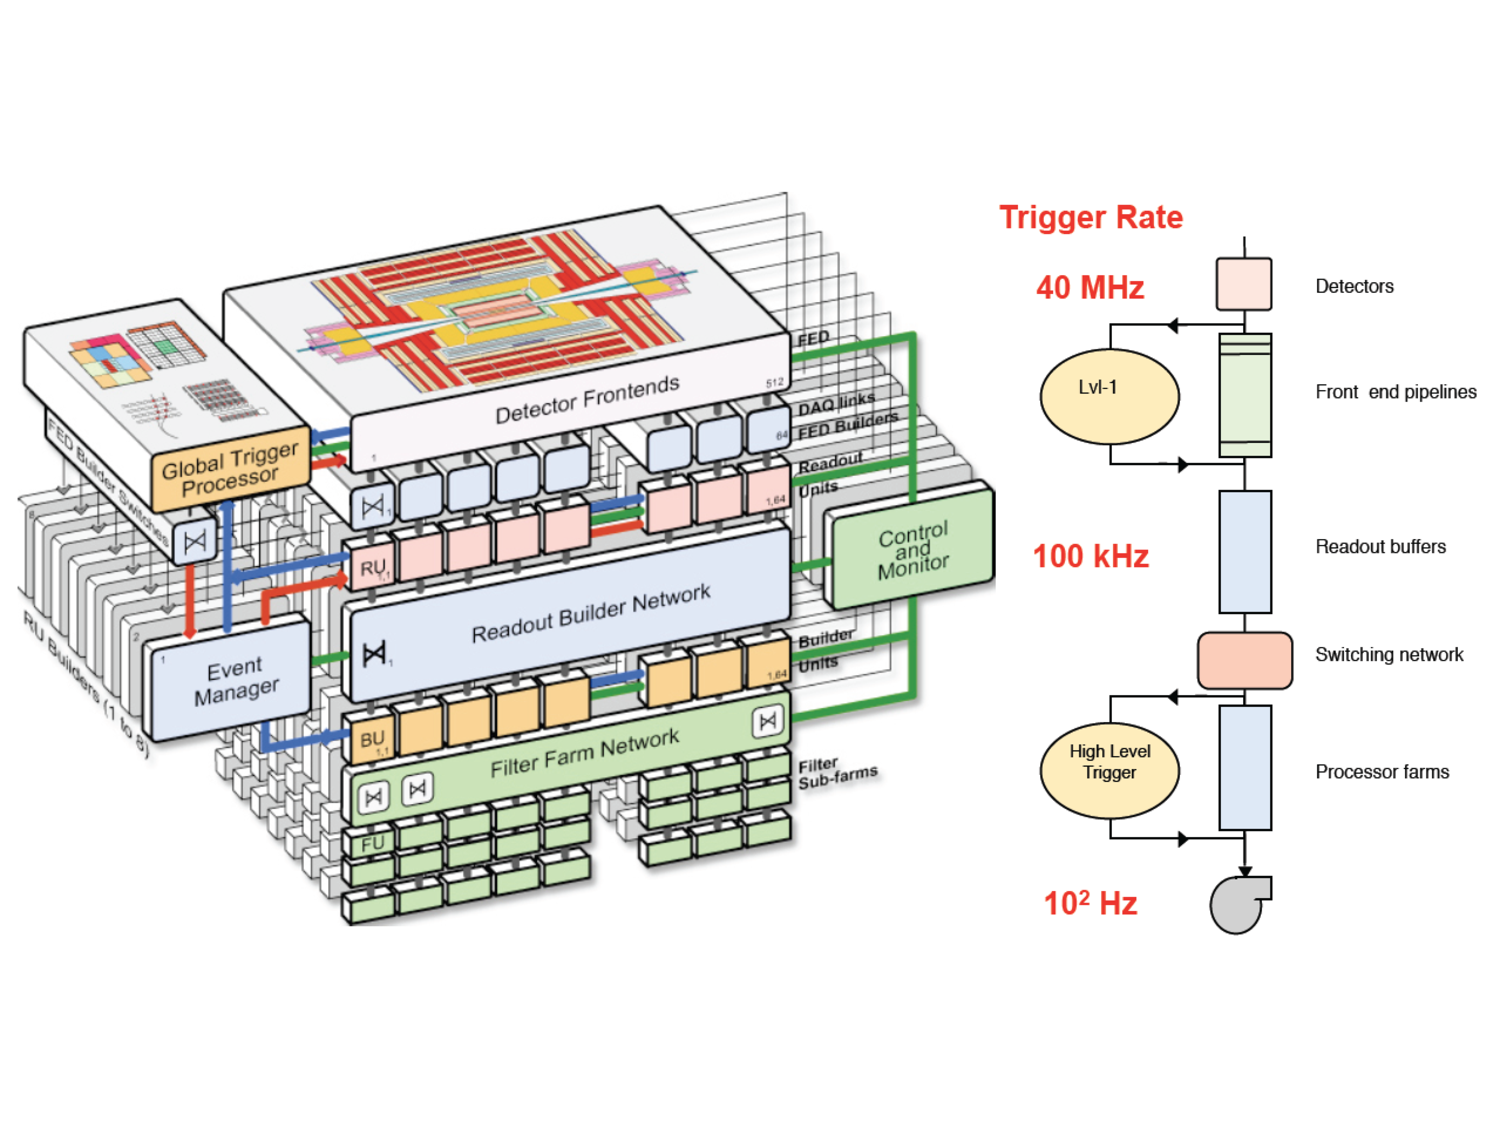
\includegraphics[width=.9\textwidth]{figs/CMSTrigger.pdf}
	\caption{CMS DAQ Architecture. The size  of the event builder (72 Readout
Units, 288  Builder Units) represents one; the  system can be equipped
with up to eight slices. \label{fig:hltarc}}
	\end{center}
\end{minipage}
\begin{minipage}[t]{7.0cm}
\begin{center}
	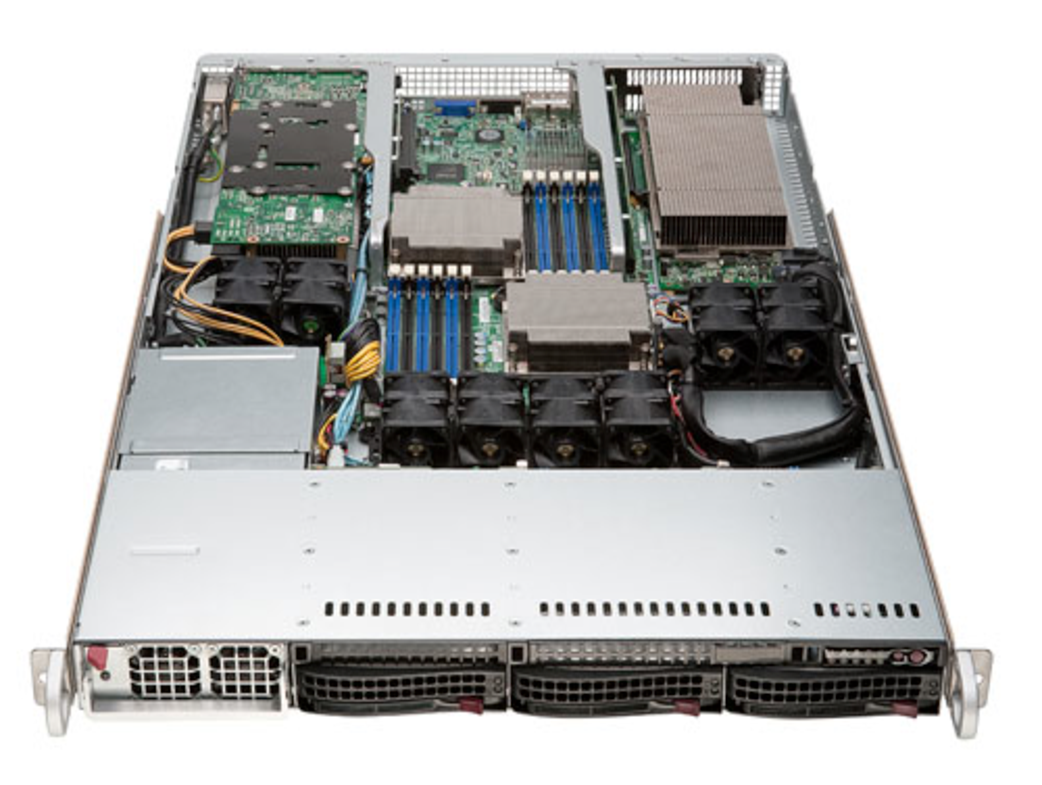
\includegraphics[width=0.8\textwidth]{figs/Tesla_M1060_1u_Super_Micro_Front_Elevated_no_cover_large.pdf}
	\caption{Integrated GPU/CPU 1U server (image courtesy of NVIDIA).   \label{fig:integratedsys}}
	\end{center}
\end{minipage}
\end{figure}

The architecture of the CMS HLT~\cite{bib:TDR2},\cite{bib:HLT} combines the flexibility gained by using the offline
reconstruction~\cite{bib:datamodel} with the robustness required for reliable online operation of the DAQ. Figure~\ref{fig:hltarc} shows 
a schematic of the architecture of the CMS DAQ system. Event fragments are read out and stored in Readout Units (RU) for each event accepted
by the Level-1 trigger. The fragments are subsequently assembled into complete events by an Event Builder through a complex of switched 
networks into event buffers (BU). The full event content is then handed to one of the HLT Filter Units (FU). The FU execute a series of 
physics reconstruction and filter algorithms and events that are found to be sufficiently interesting for offline analysis are forwarded 
to the Storage Manager (SM). The decoupling of physics algorithm execution from data flow allows each FU to continue operation, recover the
content of the problematic event, and forward it to be stored unprocessed. The FU architecture consists of 
two separate applications, the ResourceBroker, which exchanges data with the DAQ, and the EventProcessor, which integrates the reconstruction
software. Given the involved event sizes and rates, reformatting raw events consisting of a large number of small data fragments into the physical 
memory of a Filter Unit requires high bandwidth I/O, while the subsequent HLT processing is mostly CPU intensive.
The EventProcessor previously mentioned encapsulates the event processing machinery of the CMS reconstruction, providing the full flexibility 
required to execute complex physics algorithms. 

The farms of machines where these event selections are executed is a natural place where the GPUs could be integrated.
A simple solution is shown in Figure~\ref{fig:integratedsys} with a 1U server containing dual multicore CPUs and two NVIDIA Tesla GPUs. 
While this would provide a single, integrated 1U GPU/CPU server this of course implies replacing the existing servers, 
evaluating the new power consumption, and the cost of these servers relative to any other options.



\section{Inner Tracker}

Both the CMS and ATLAS inner tracker include a silicon pixel detector and a silicon strip detector.
All tracker layers provide two-dimensional hit position measurements, but only the pixel tracker
 and a subset of the strip tracker layers provide three dimensional hit position measurements.
Only the CMS tracker is considered however the detector performances are comparable
in CMS/ATLAS experiments and the tracking algorithm and results discussed are applicable for both of 
these experiments as well. The CMS pixel detector includes three barrel layers and two forward disks
on either end of the detector surrounded by  ten strip detectors barrel layers plus three 
inner disks and nine forward disks at each end of the detector.
Owing to the strong magnetic field and the high granularity of the silicon tracker, 
promptly produced charged particles with transverse momentum $pT = 100$ GeV/c are reconstructed 
with a resolution in pT of 1.5\% and in transverse impact
parameter d0 of 15 mm. The track reconstruction algorithms are able to reconstruct displaced
tracks with transverse impact parameters up to 25 cm from particles decaying up to 50 cm
from the beam line. The performance of the track reconstruction algorithms has been studied
with data [11]. The silicon tracker is also used to reconstruct the primary vertex position with
 a precision of $\sigma_d = 20$ mm in each dimension. 

%% Paul maybe add a pic of the cms tracker and a 2D track reco in the tracker for the kalman fit
%% and reference to them in these 2 sections
\section{Current Tracking Algorithm}

The CMS track reconstruction uses an iterative algorithm, with earlier iterations searching for tracks that are more easily found 
(relatively higher $p_T$ tracks close to the interaction region). The hits in these tracks are then removed, allowing later iterations 
to search for lower momentum or highly displaced tracks without the combinatorial possibilities becoming too large. Each iteration 
consists of four steps. First, a seed, consisting of either three hits or two hits and a primary vertex constraint, is constructed 
to create an initial estimate of the trajectory parameters for the track. Second, track finding is performed using a global Kalman 
fiter.~\cite{Fruhwirth:1987fm} This step performs a fast propagation of the track candidate to propagate the track through the
 layers of the detector, search for compatible nearby hits, and attach them to the candidate. After all candidates in this step have
 been found, the track candidate collection is then cleaned to remove duplicate tracks or tracks which share a large number of hits. 
The third step is to perform a full Kalman fit over the whole track to obtain the best estimate of the track parameters at all points 
along the trajectory. The filter begins at the innermost hits, and then iterates outward through each hit to update the track trajectory 
estimate and its uncertainty. After this first fit is complete, a smoothing stage is then performed running backwards from the last hit 
to apply the information from the later hits to the earlier ones. This step uses a Runge-Kutta propagator to account for the effect of 
material interactions and an inhomogenous magnetic field. Finally, track selection requirements are applied to reduce the fake rate of the resulting track candidates.






\section{Proposed Fast Tracking Algorithm}

One possible application of the GPU enabled parallelism would be to
accelerate the performance of the existing combinatorial track finder.
Since the iterative Kalman process for each track is largely independent of the other tracks,
parallelization should not be conceptually difficult. However, an additional motivating 
force behind the use of GPU in the HLT is to be able to investigate the possibility of 
running trigger algorithms which are dramatically and qualitatively different in nature 
to enhance the discovery potential.

As an example, the Hough Transform is a well known algorithm used in various machine
vision applications that differs from the Kalman approach in that it does not operate on
localized features of a data set.  Rather the technique is in some sense more
holistic, operating on an entire image as a whole. 
% Patrick a comment to account to the fact that would not need large MEM to move around to process the
% large amount of data is required here
The technique is described at length in existing literature\cite{bib:HT1},\cite{bib:HT2},
 but the concept as it would be applicable to the
tracking problem is to consider the parameterization of any given track.  Any given hit
observed in the detector, for example the simulated straight line track data shown in Figure~\ref{fig:hits}, 
can correspond to many different possible tracks in parameter space as shown in Figure~\ref{fig:accumulator}.  
When integrated over the entire data set, peaks appear in parameter space at the values corresponding to the actual, 
physical trajectories as shown in Figure~\ref{fig:tracks}.

\begin{figure}[!Hhtb]
\begin{minipage}[t]{4.9cm}
\begin{center}
	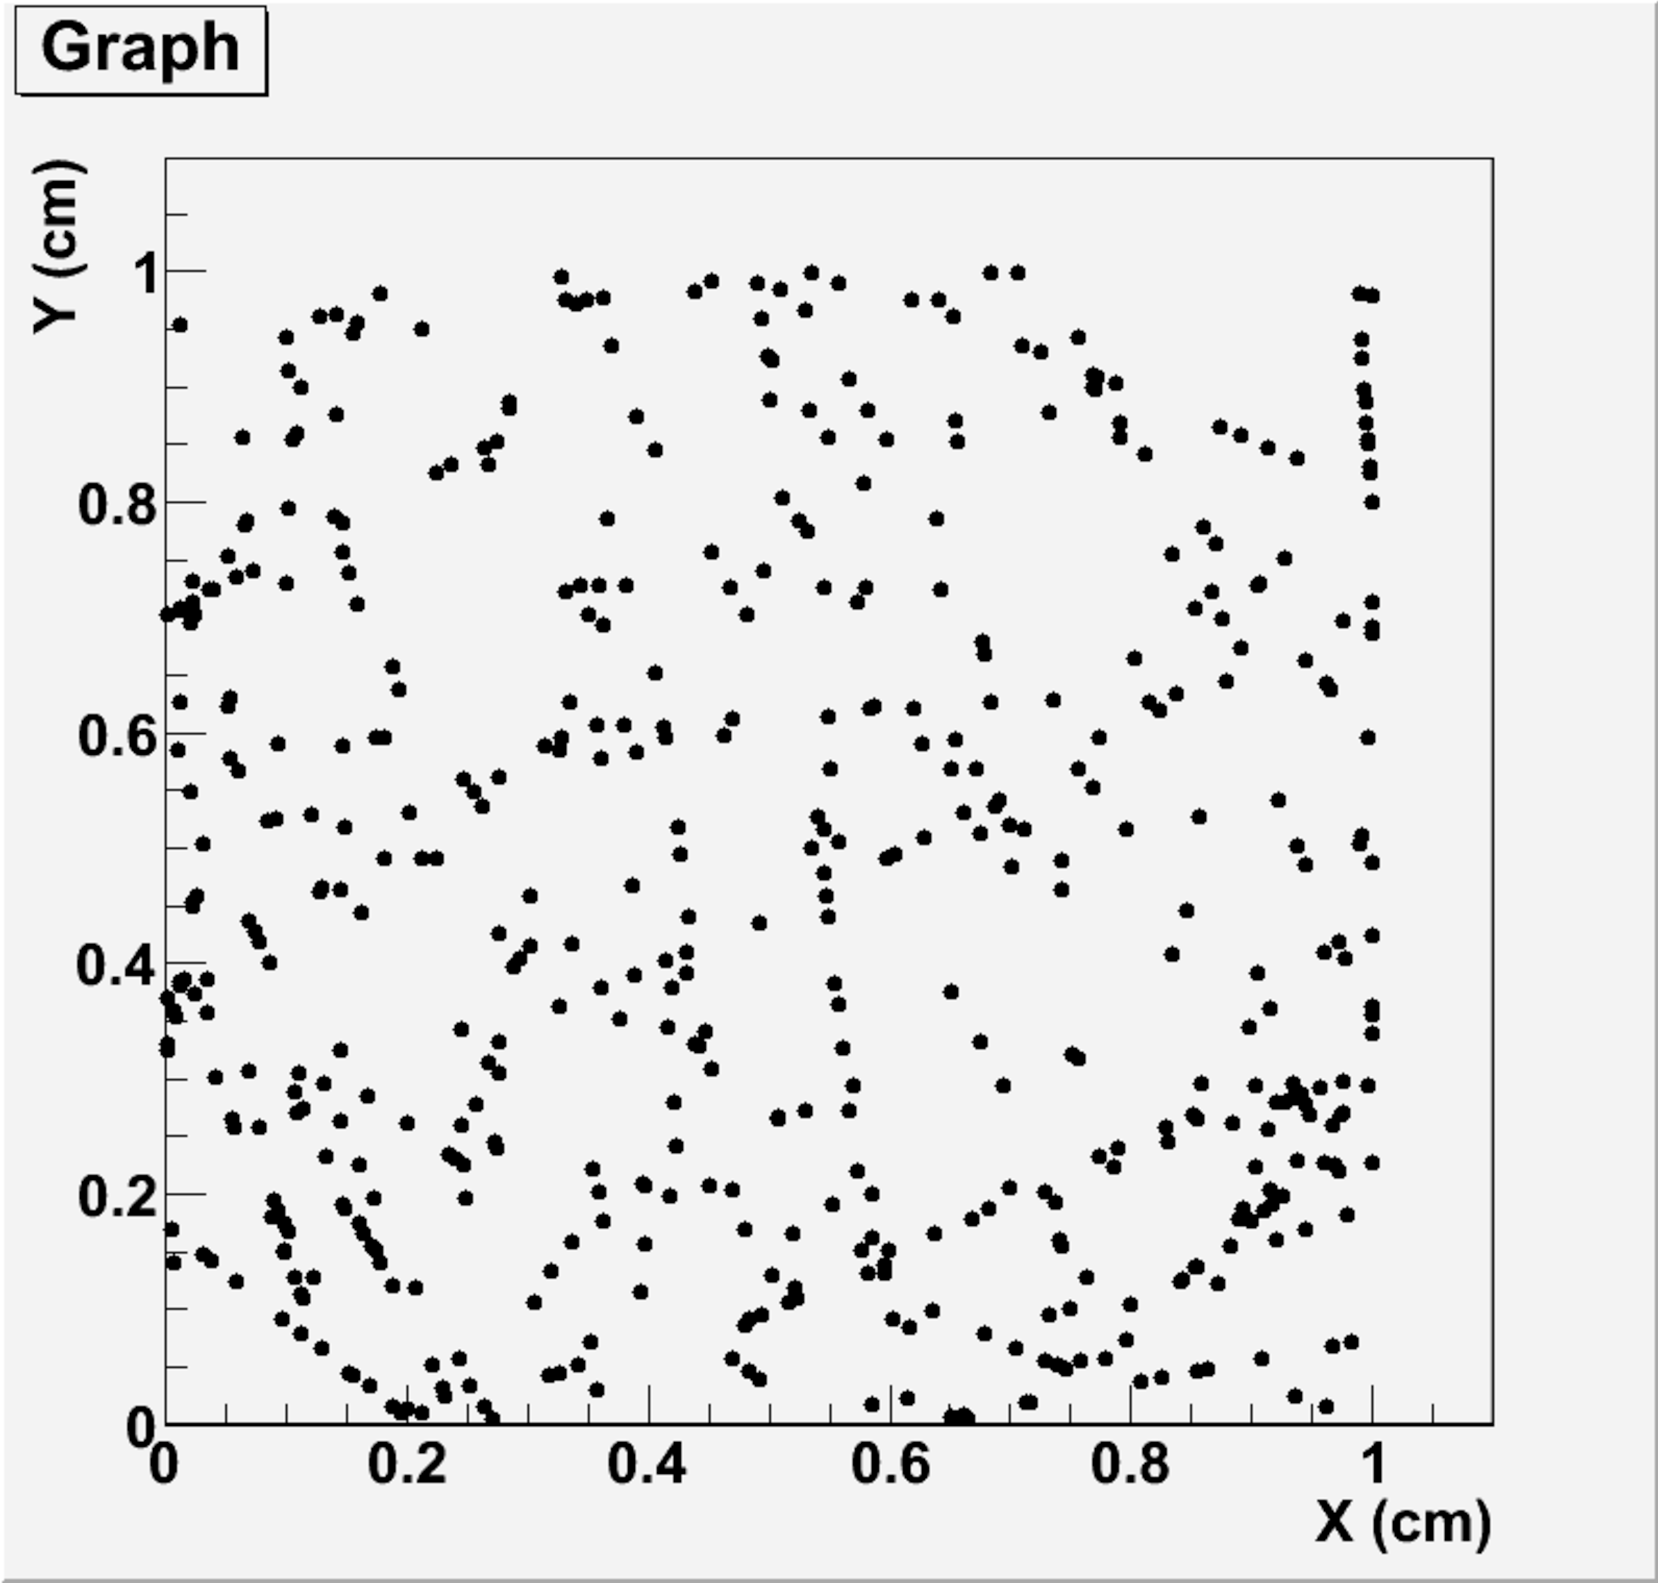
\includegraphics[width=1.\textwidth]{figs/50events_hits.pdf}
	\caption{Simulated event made up of 50 straight line tracks, with 10 hits per track. \label{fig:hits}}
	\end{center}
\end{minipage}
\begin{minipage}[t]{4.9cm}
\begin{center}
	\includegraphics[width=0.95\textwidth]{figs/50events_accumulator.pdf}
	\caption{Each hit results in a sinusoidal line in the parameter space.  Locations where many 
of these sinusoidal lines cross are likely to be tracks in the original data.  \label{fig:accumulator}}
	\end{center}
\end{minipage}
\begin{minipage}[t]{4.9cm}
\begin{center}
	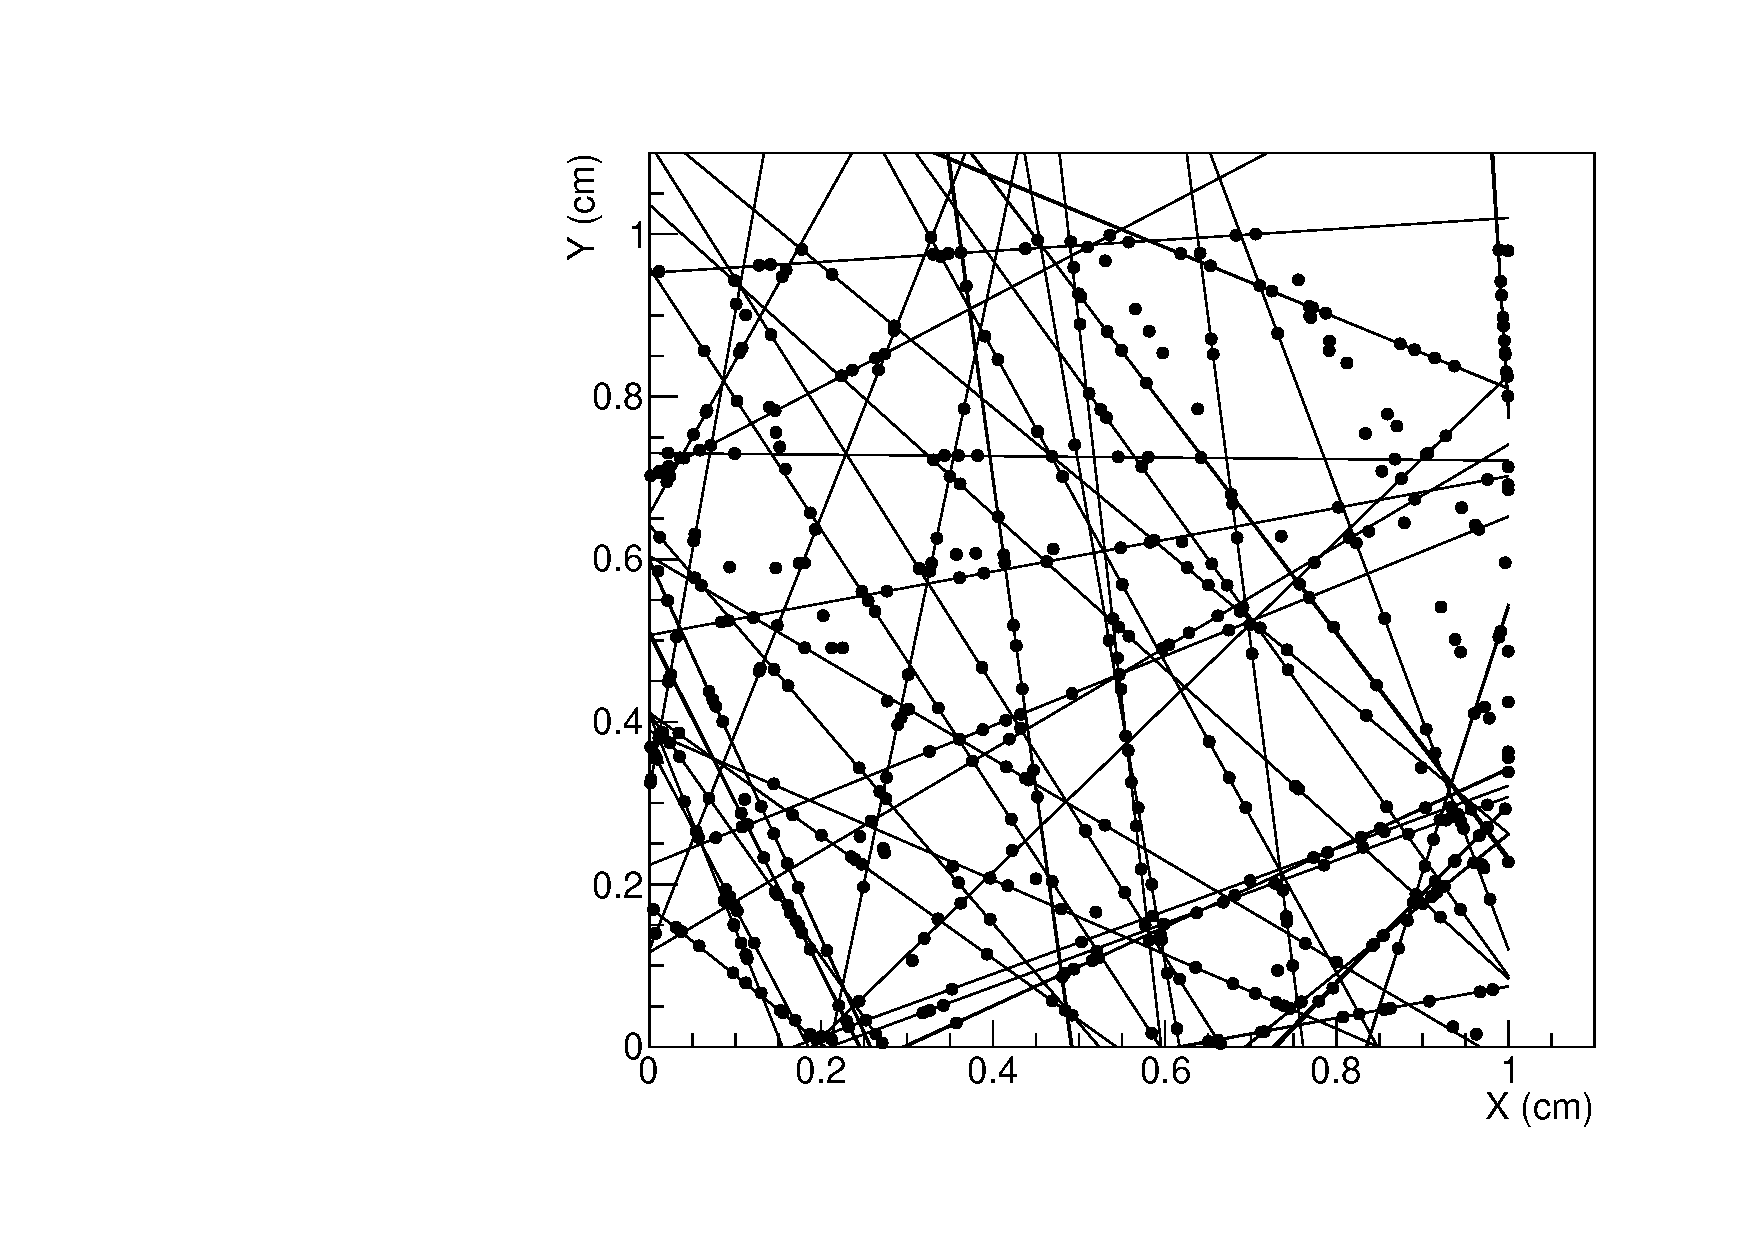
\includegraphics[width=1.\textwidth]{figs/50events_hits_tracks.pdf}
	\caption{Candidate tracks identified from finding local maxima in the parameter space.  \label{fig:tracks}}
	\end{center}
\end{minipage}
\end{figure}

\section{Preliminary Results}

As was briefly described previously, the traditional combinatoric track finder  approach implicitly depends on various assumptions and
constraints on the phase space of the seed tracks, with one of the most significant
results being suppression of displaced vertices and other odd tracks due to extensice processing time.
 It is hoped that a more holistic algorithm
can be used to supplement the existing tracking algorithm in a significant way.
As a demonstration of this a simple tracking algorithm based on the Hough Transform was developed 
and run against a stand alone Monte Carlo simulation with a simple tracker geometry file. 
The preliminary investigation was performed using Intel multicore CPUs and NVIDIA Tesla C2075 and K20c GPUs.

The Hough Transform algorithm is not trivial to implement in parallel because the computation of the parameter space is subject to race
conditions whereby it is not necessarily safe to have multiple threads arbitrarily make updates as hits are processed.  In the interest of time
and having an unbiased performance comparison for the GPU implementation it would have been preferable to use the CPU implementation of the Hough Transform 
from the Intel Performance Primitives (IPP) library.  However, it was observed that the implementation in IPP is not parallelized and so to provide a more 
fair performance comparison a parallel implementation of the Hough Transform for the CPU has been developed as part of this work.  This CPU implementation is
 parallelized using OpenMP threads and speedups of 2.6 - 3.6 were achieved on a Intel Core i7-3770 (Ivy Bridge, Quad Core, 3.4 GHz) processor.  The CPU used 
for the performance results is physically a quad core CPU but supports up to two threads per physical core using Simultaneous Multithreading (SMT), 
with the Intel implementation of SMT known as HyperThreading (HT).  SMT did not show any performance advantage for this application because the speedup
 actually dropped as the number of threads exceeded the number of physical cores.  For the GPU implementation, performance results for the two most recent 
generations of NVIDIA GPUs are shown in Figure~\ref{fig:TimePerformance}.  Note that the GPU implementation is up to 100x faster than the best multithreaded CPU implementation.

\begin{figure}[!Hhtb]
%\begin{minipage}[t]{8.0cm}
%\begin{center}
%	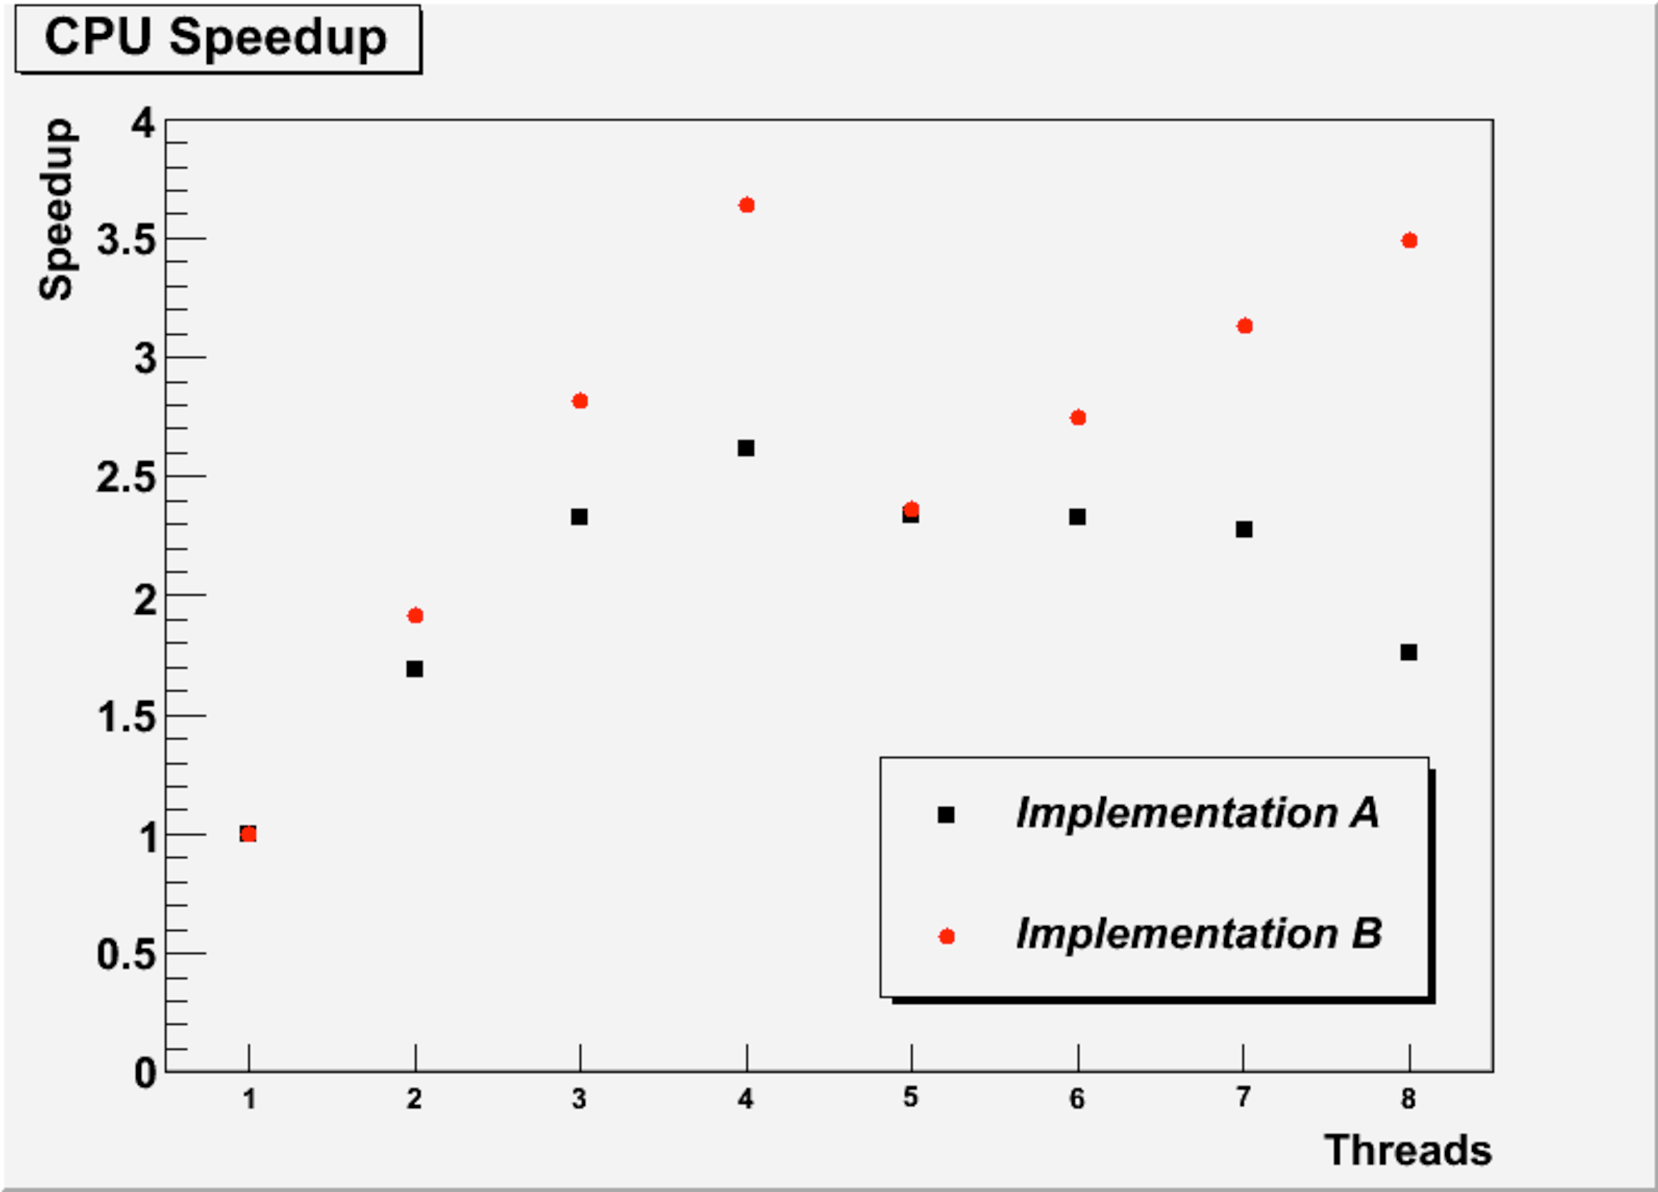
\includegraphics[width=0.9\textwidth]{figs/cpu_speedup.pdf}
%	\caption{Speedup for two different implementations of the Hough Transform.  Parallelization uses OpenMP on an Intel Core i7-3770 (Ivy Bridge, Quad Core, 3.4GHz)  \label{fig:cpu_speedup}}
%	\end{center}
%\end{minipage}
\begin{minipage}[t]{8.0cm}
\begin{center}
	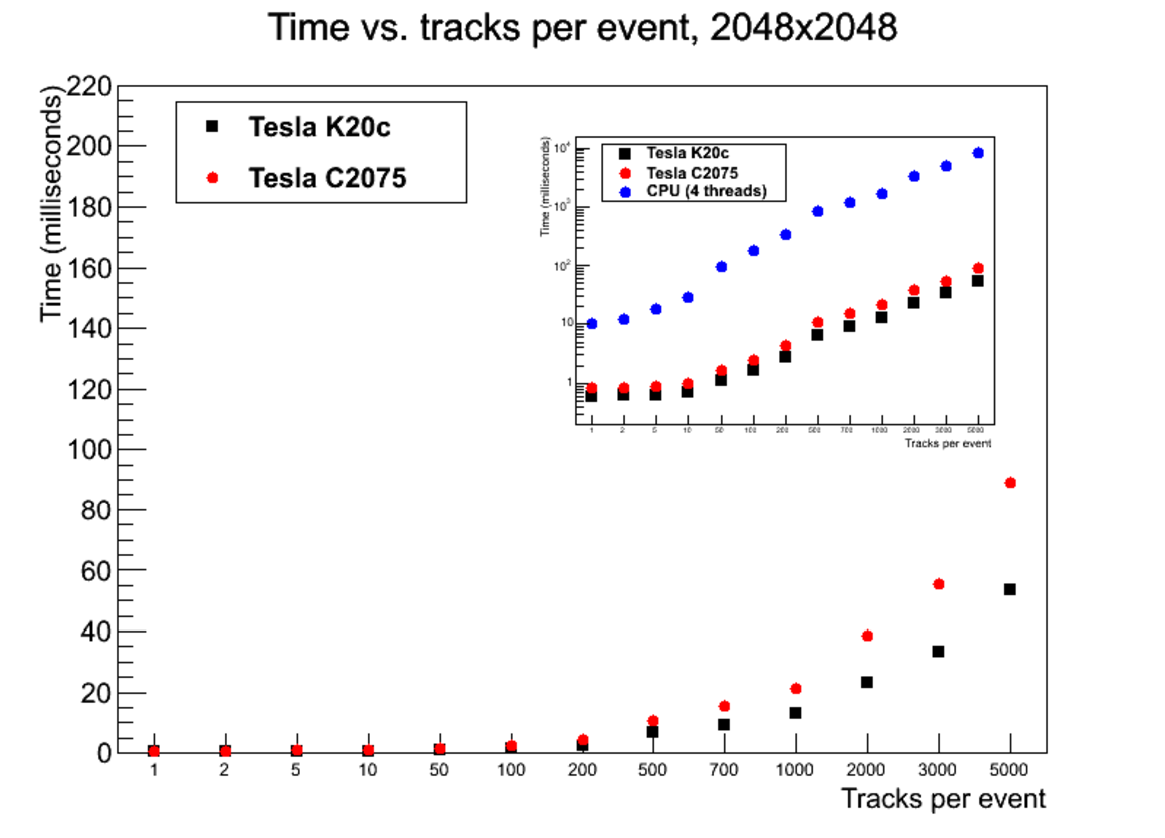
\includegraphics[width=0.9\textwidth]{figs/TimePerformance.pdf}
	\caption{Performance comparison of the Intel CPU (using 4 threads), NVIDIA Tesla C2075, and NVIDIA Tesla K20c. \label{fig:TimePerformance}}
	\end{center}
\end{minipage}
\begin{minipage}[t]{8.0cm}
\begin{center}
	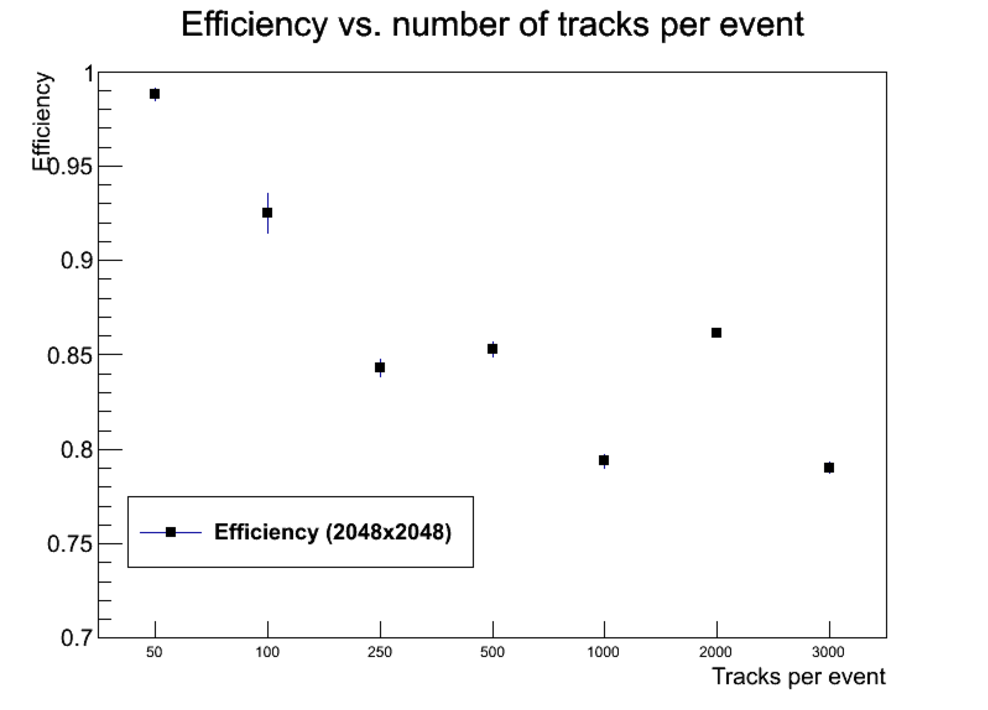
\includegraphics[width=0.9\textwidth]{figs/Eff.pdf}
	\caption{Efficiency as the number of tracks per event is varied.  \label{fig:Eff}}
	\end{center}
\end{minipage}
\end{figure}

Although the Hough Transform is most often associated with finding straight lines in data it is applicable to any feature which can be represented 
by a finite number of parameters.  For example, circles of unknown location and radius and location can be identified in a three dimensional parameter 
space representing the x and y location of the center plus a third parameter for the radius.  Figures~\ref{fig:mc_hits} and~\ref{fig:mc_tracks} show 
an example of results for our Hough Transform implementation used for identifying curved tracks.  Similar to straight tracks, this curved track 
implementation is in terms of a two dimensional parameter space by constraining the tracks to pass through the interaction point.  
The computational cost of the Hough Transform is strongly dependent on the total number of parameters while the details of the particular parameterization
 has essentially no effect on the performance.

\begin{figure}[!Hhtb]
\begin{minipage}[t]{8.0cm}
\begin{center}
	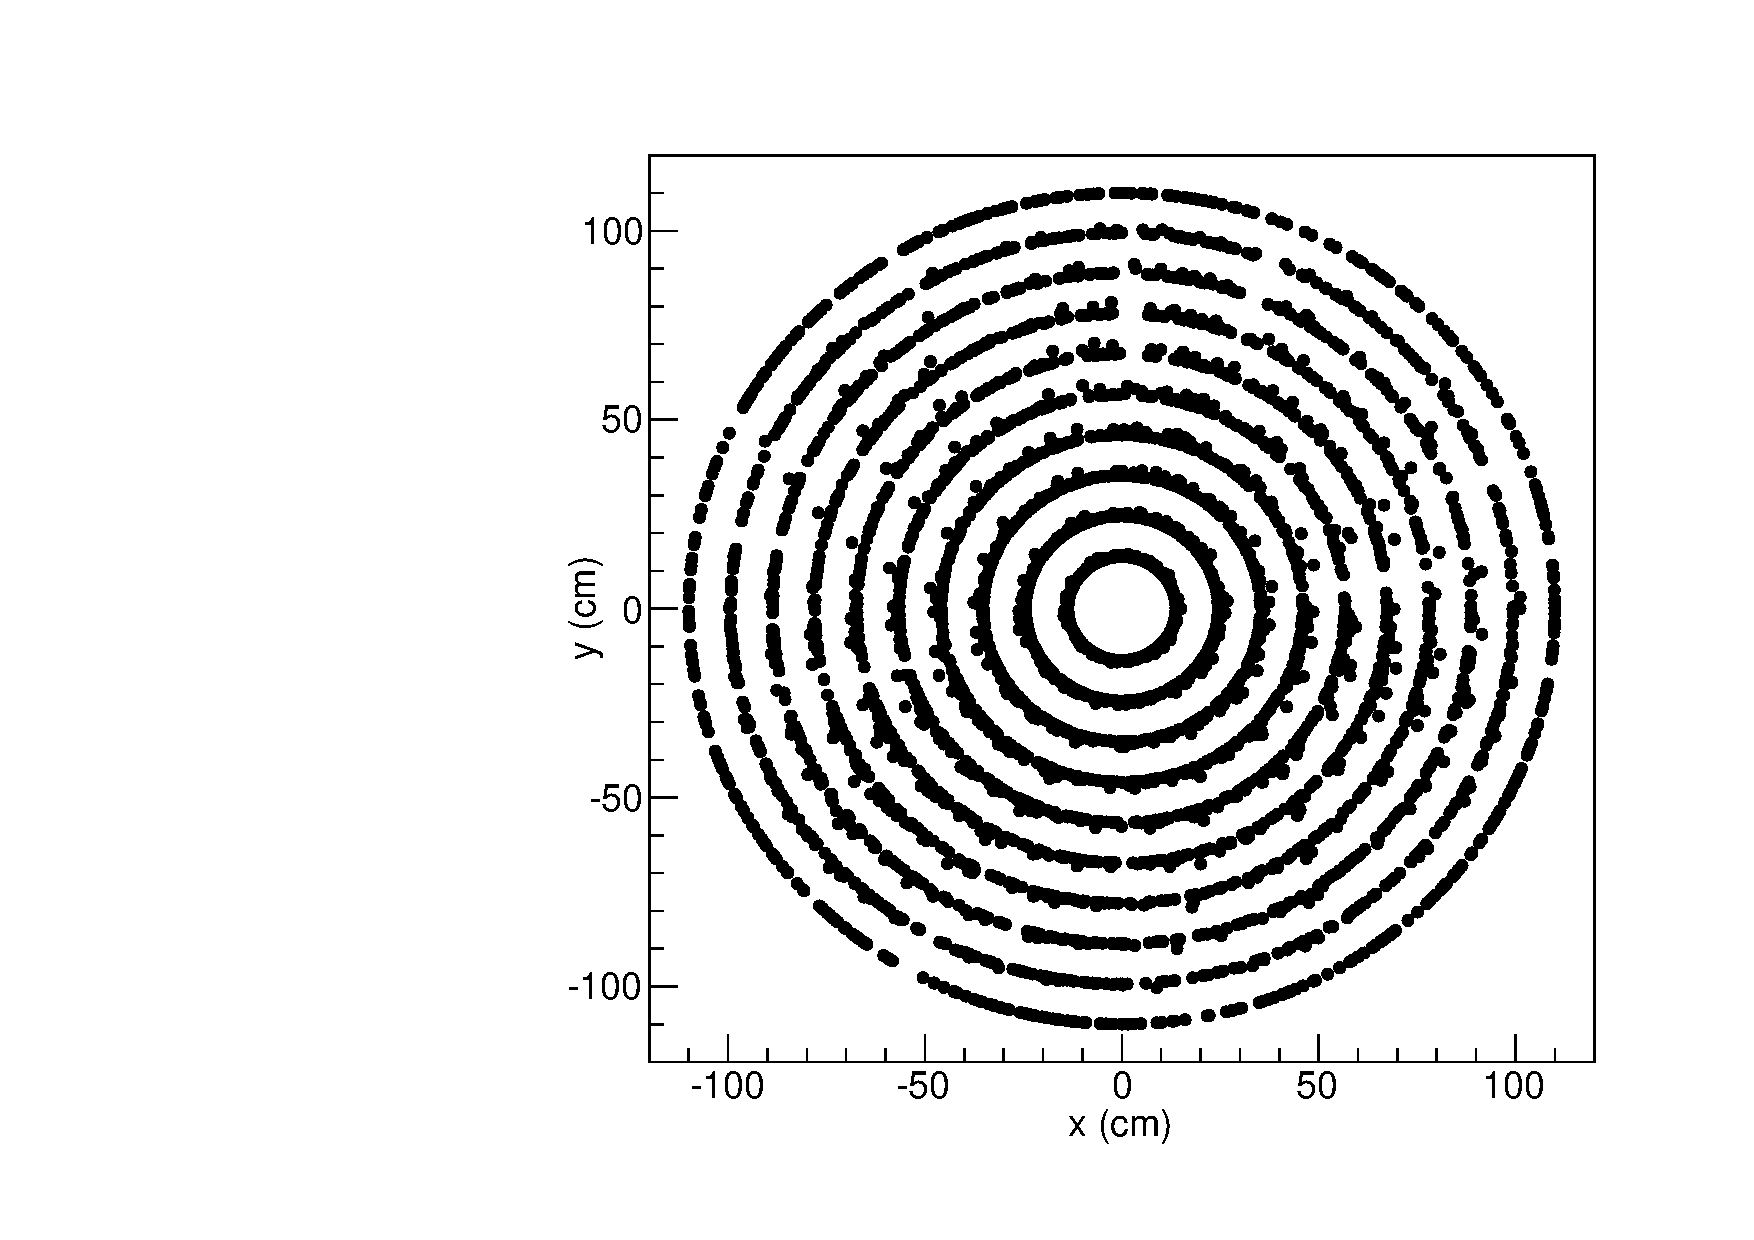
\includegraphics[width=0.9\textwidth]{figs/curved_500events_hits.pdf}
	\caption{Monte Carlo data for curved tracks originating from the interaction point. \label{fig:mc_hits}}
	\end{center}
\end{minipage}
\begin{minipage}[t]{8.0cm}
\begin{center}
	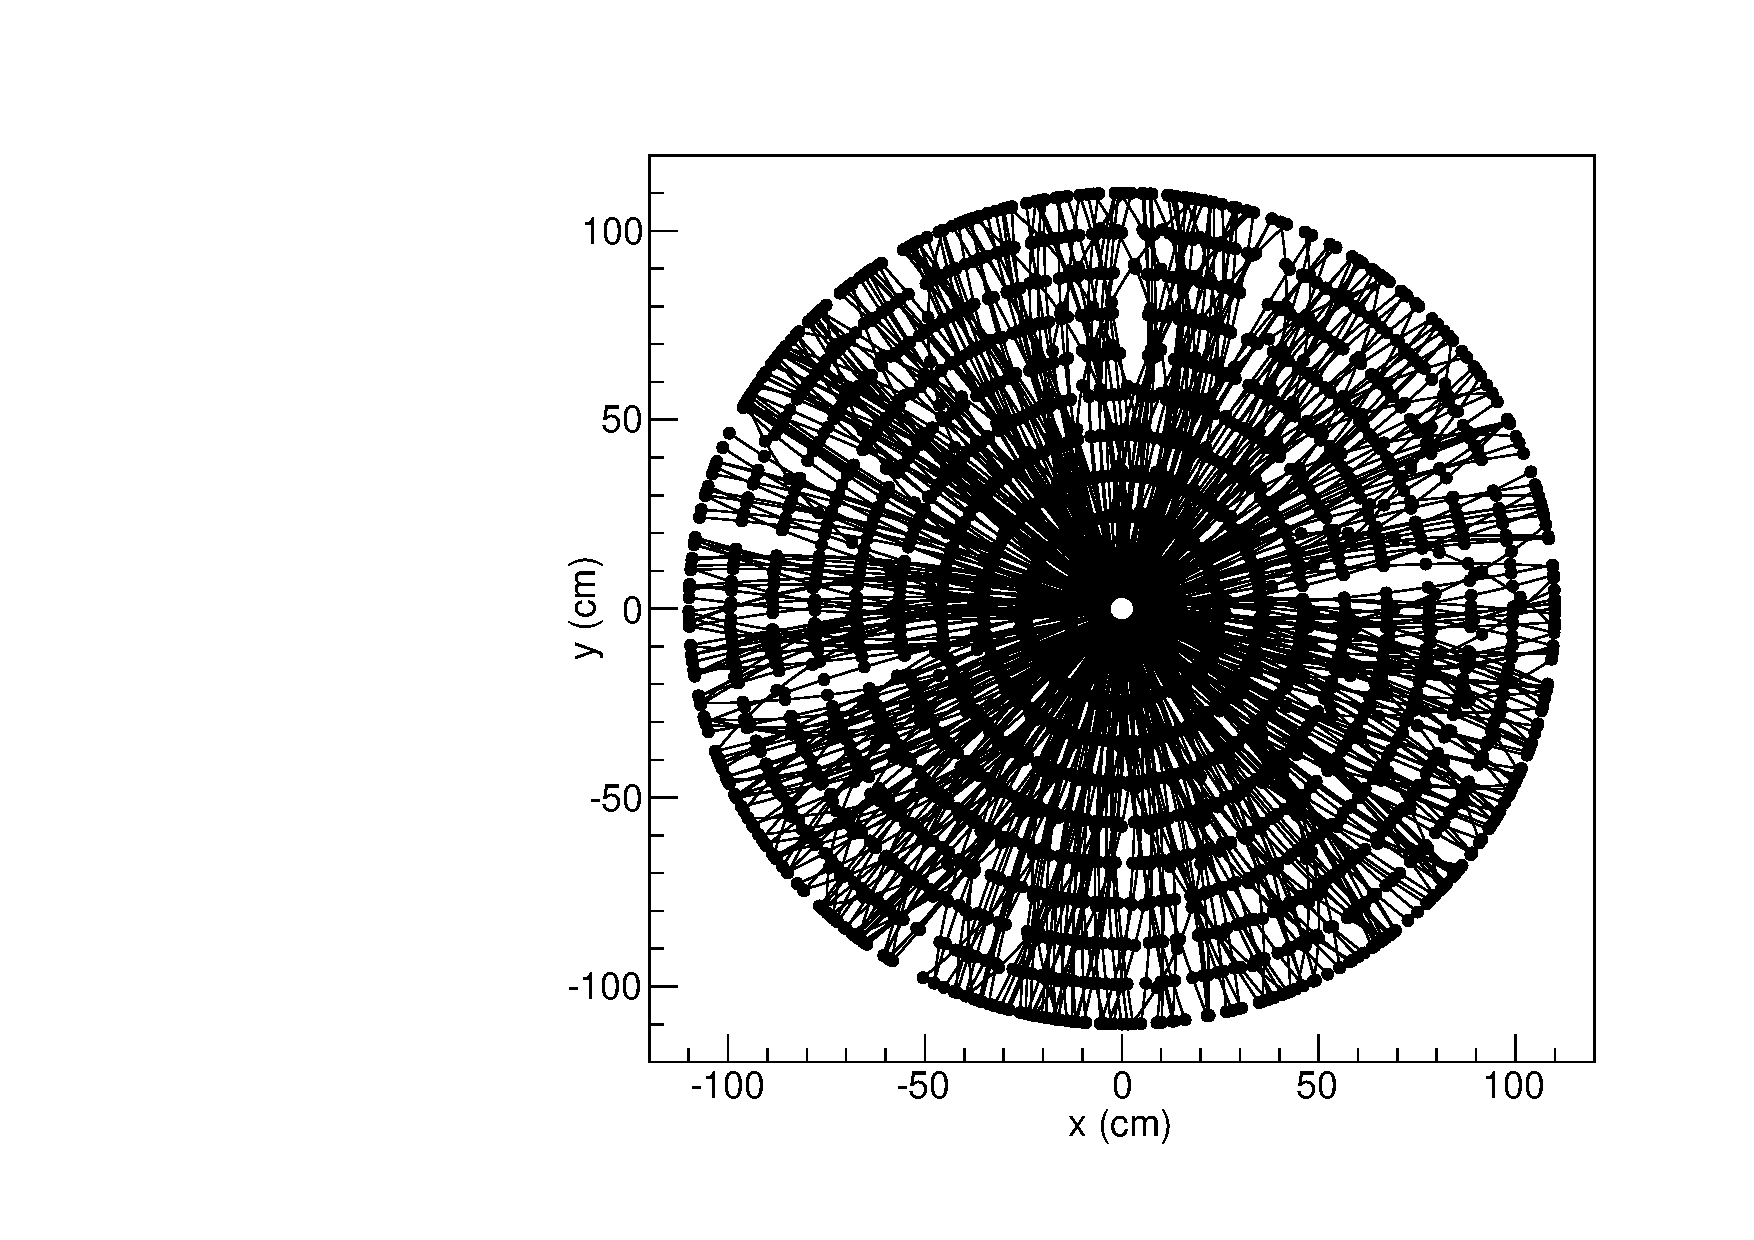
\includegraphics[width=0.9\textwidth]{figs/curved_500events_hits_tracks.pdf}
	\caption{Curved tracks identified using the Hough Transform.  \label{fig:mc_tracks}}
	\end{center}
\end{minipage}
\end{figure}

While the Hough Transform is a critical part of the proposed tracking algorithm, it is not the only aspect of the computation.  After candidate tracks have been 
identified from analysis of the parameter space it may be necessary to perform a fit of the hits to the candidate tracks.  This fitting operation is well suited
 to parallelization on the GPU, but the performance results in Figures~\ref{fig:TimeVsThreads} and~\ref{fig:TimeVsTracks} shows that a multithreaded CPU implementation
 requires only a few milliseconds.  In comparison the Hough Transform on the GPU requires many tens of milliseconds so the fitting operation is relatively low priority f
or performance optimization.  If or when fitting became a significant performance bottleneck it could certainly be run on the GPU to further increase performance.

\begin{figure}[!Hhtb]
\begin{minipage}[t]{8.0cm}
\begin{center}
	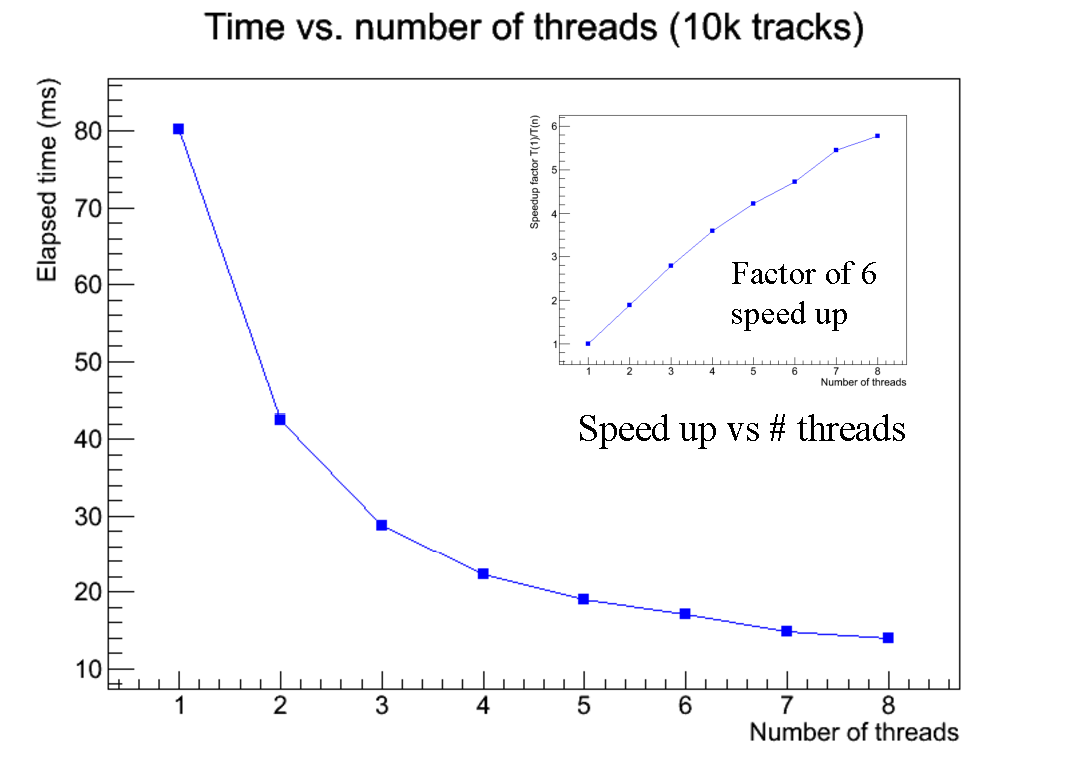
\includegraphics[width=0.9\textwidth]{figs/TimeVsThreads.pdf}
	\caption{CPU speedup for the fitting computation. \label{fig:TimeVsThreads}}
	\end{center}
\end{minipage}
\begin{minipage}[t]{8.0cm}
\begin{center}
	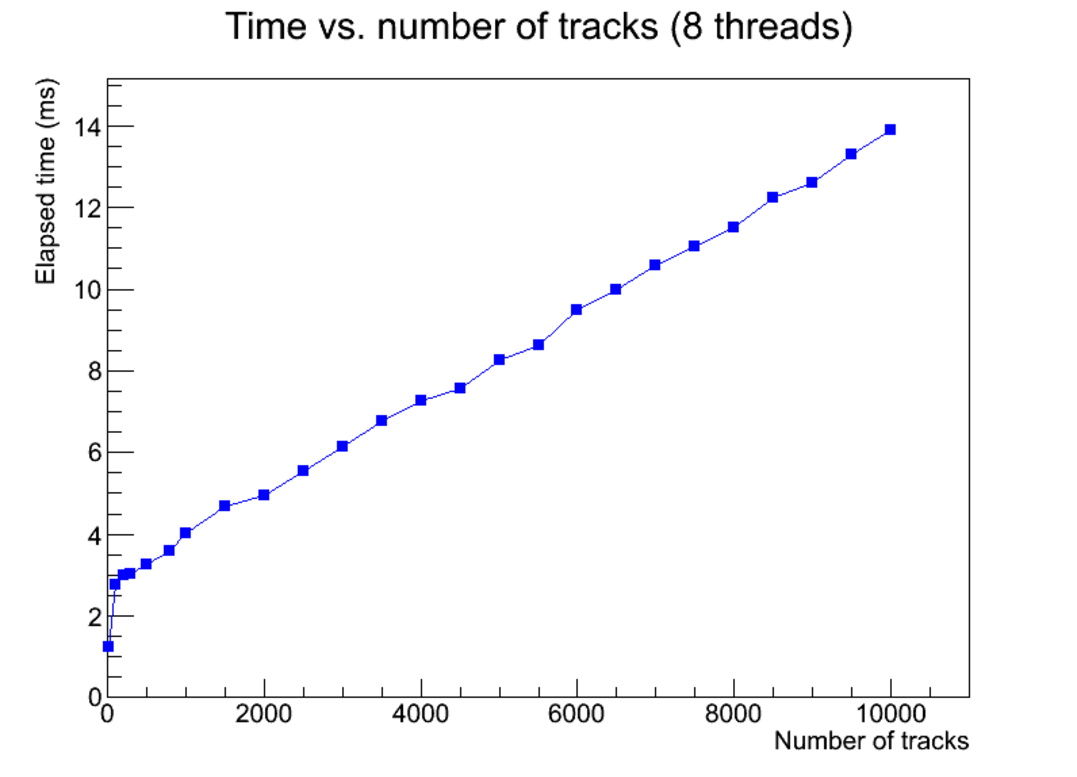
\includegraphics[width=0.9\textwidth]{figs/TimeVsTracks.pdf}
	\caption{Time required for the fitting computation as the number of tracks is varied.  \label{fig:TimeVsTracks}}
	\end{center}
\end{minipage}
\end{figure}

\section{New Tracking Capabilities}

The ability to handle displaced vertices provides the opportunity to identify interesting new physics such as non prompt jets and black holes.  
To demonstrate this capability consider the tracks in Figure~\ref{fig:jet1_tracks} which originate from a displaced vertex.  
Again the Hough Transform is applied to the corresponding hits making up these tracks to generate the parameter space in 
Figure~\ref{fig:jet1_accumulator}.  Recall that the parameter space identifies candidate tracks as locations where many 
sinusoids cross one another.  In Figure~\ref{fig:jet1_accumulator} the locations of these crossings are visually apparent 
as the bright spots in the parameter space.  However, the analysis is taken one step further by noting that the crossings
 all lie along a single sinusoidal curve in the parameter space.  This single sinusoidal curve has been isolated in 
Figure~\ref{fig:jet1_vertex} and is significant because that one sinusoidal curve in the parameter space corresponds to 
a point in the original x-y space.  More importantly that point in the original x-y space corresponds to the vertex of the displaced jet. 
 And interestingly the most convenient way to implement this process is to use the Hough Transform a second time, this time applying 
it not to the hits in the x-y space but the crossings in the parameter space.  Using the appropriate parameterization to look for sinusoidal curves
 instead of straight lines the curve in Figure~\ref{fig:jet1_vertex} is identified and the vertex of the jet is now located.  
Figures~\ref{fig:jet2_tracks} -~\ref{fig:jet2_vertex} illustrate the same technique applied to an event with multiple displaced jets.

\begin{figure}[!Hhtb]
\begin{minipage}[t]{4.9cm}
\begin{center}
	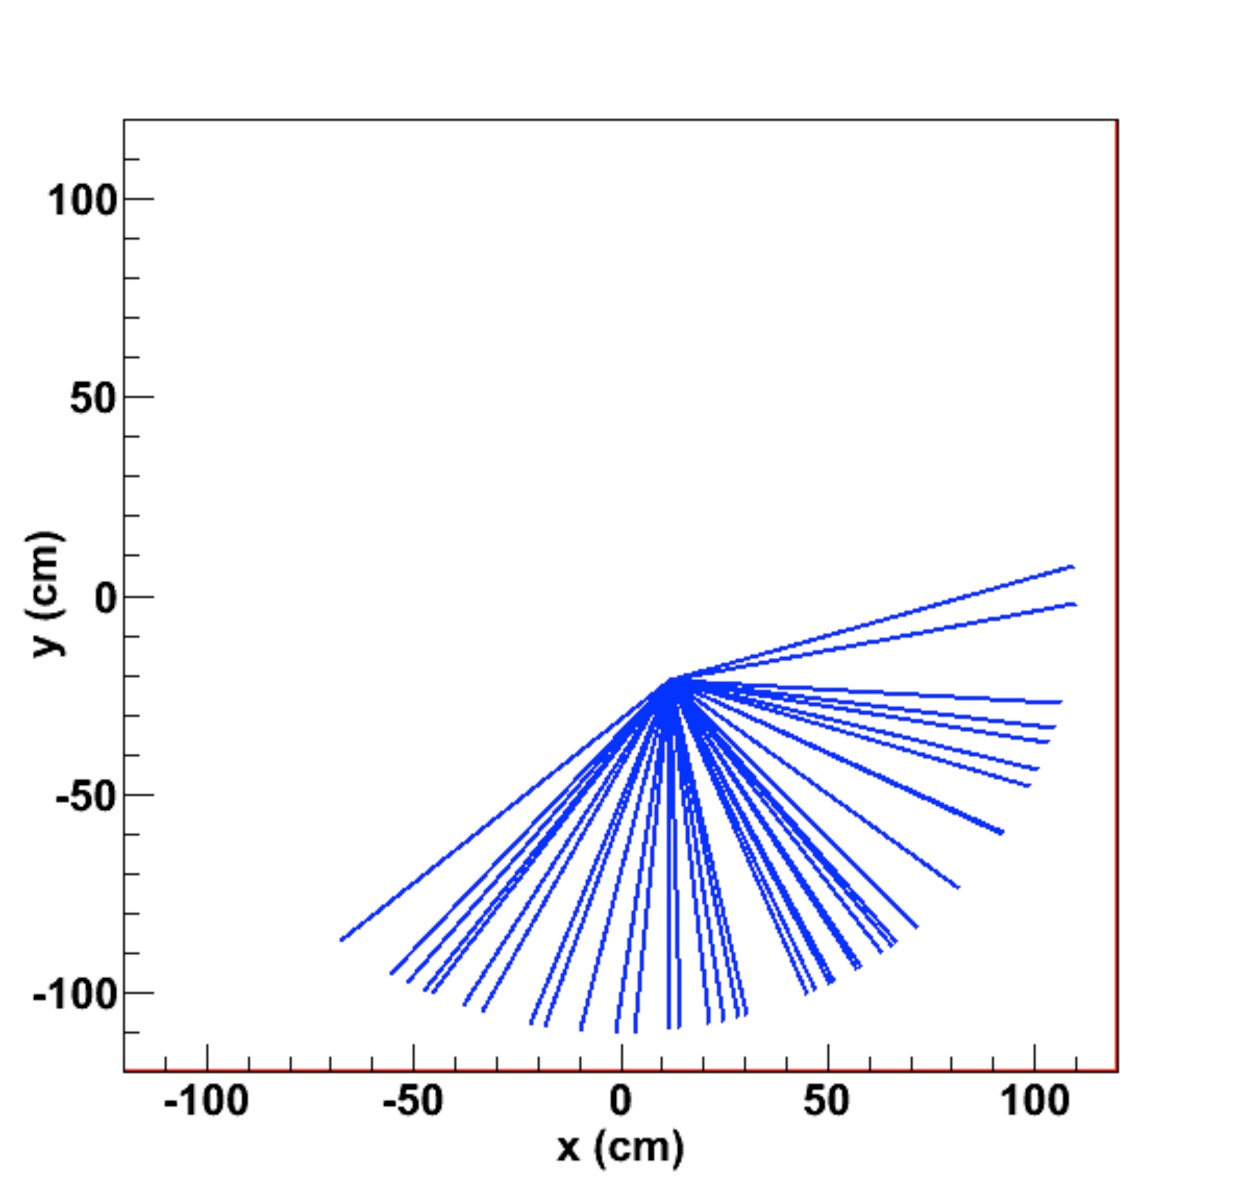
\includegraphics[width=1.\textwidth]{figs/jet1/tracks.pdf}
	\caption{Tracks originating from a displaced jet. \label{fig:jet1_tracks}}
	\end{center}
\end{minipage}
\begin{minipage}[t]{4.9cm}
\begin{center}
	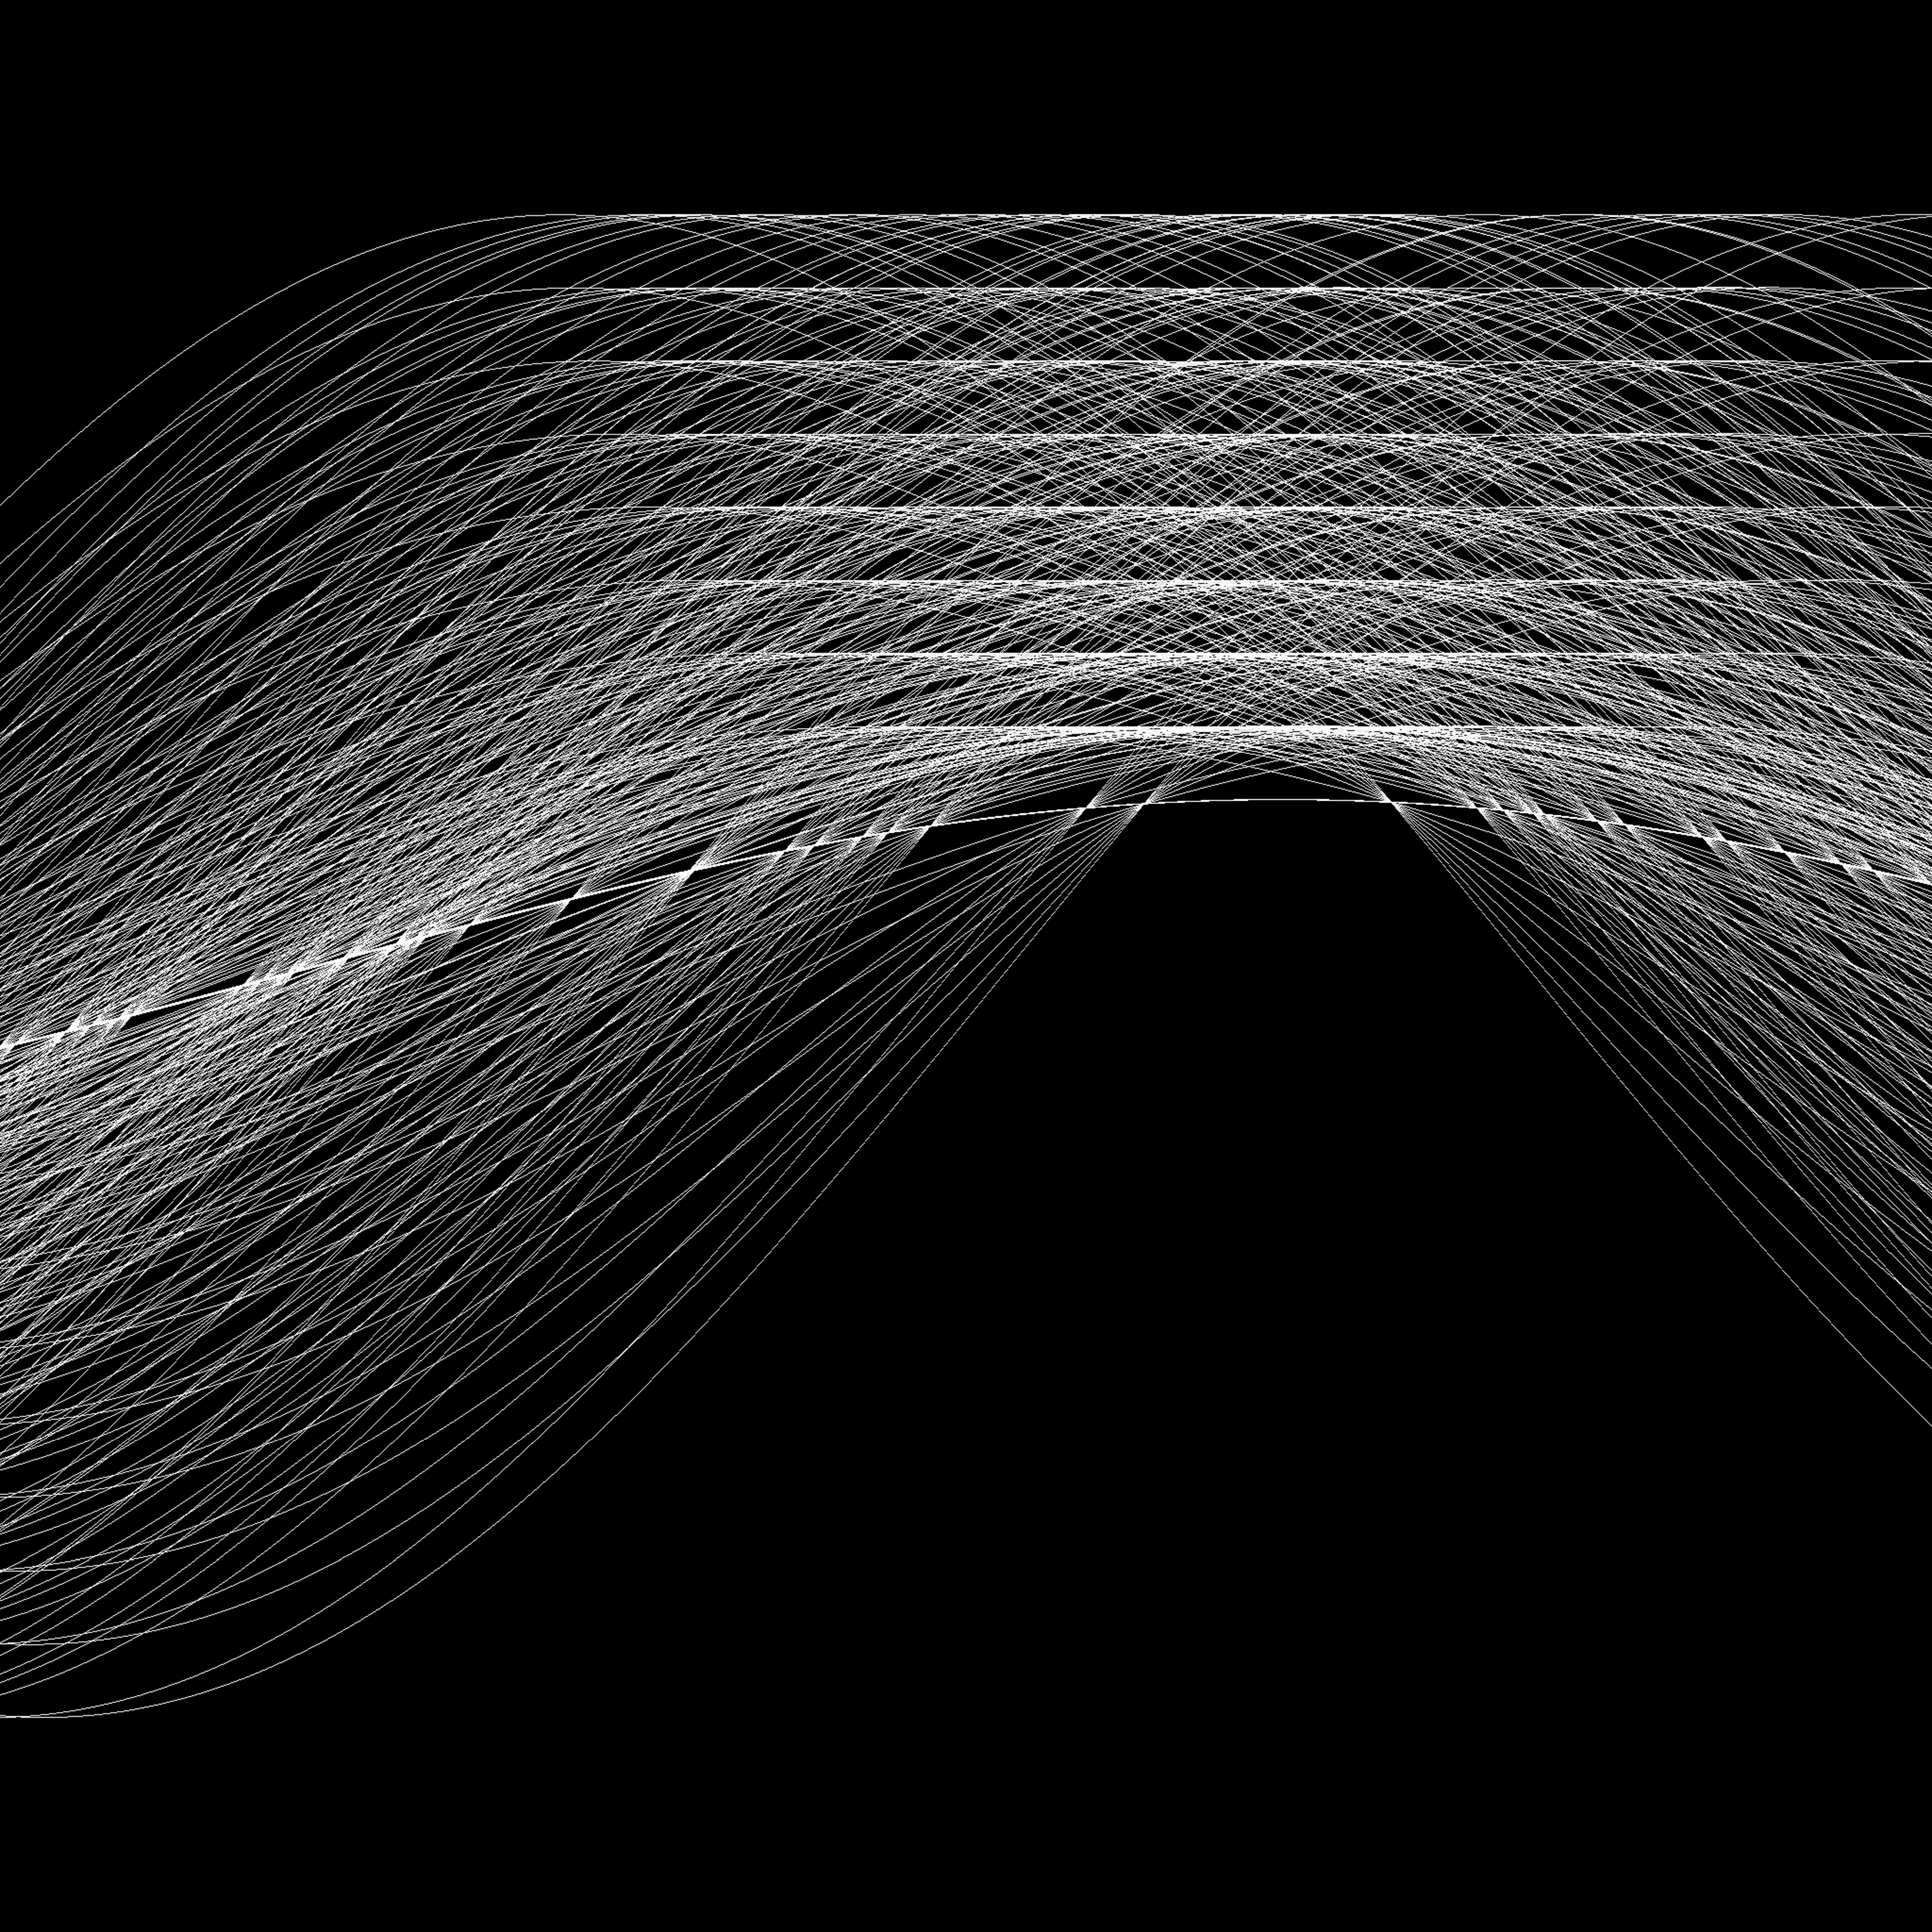
\includegraphics[width=0.88\textwidth]{figs/jet1/accumulator.pdf}
	\caption{Parameter space shows the maxima are on a single sinusoid.  \label{fig:jet1_accumulator}}
	\end{center}
\end{minipage}
\begin{minipage}[t]{4.9cm}
\begin{center}
	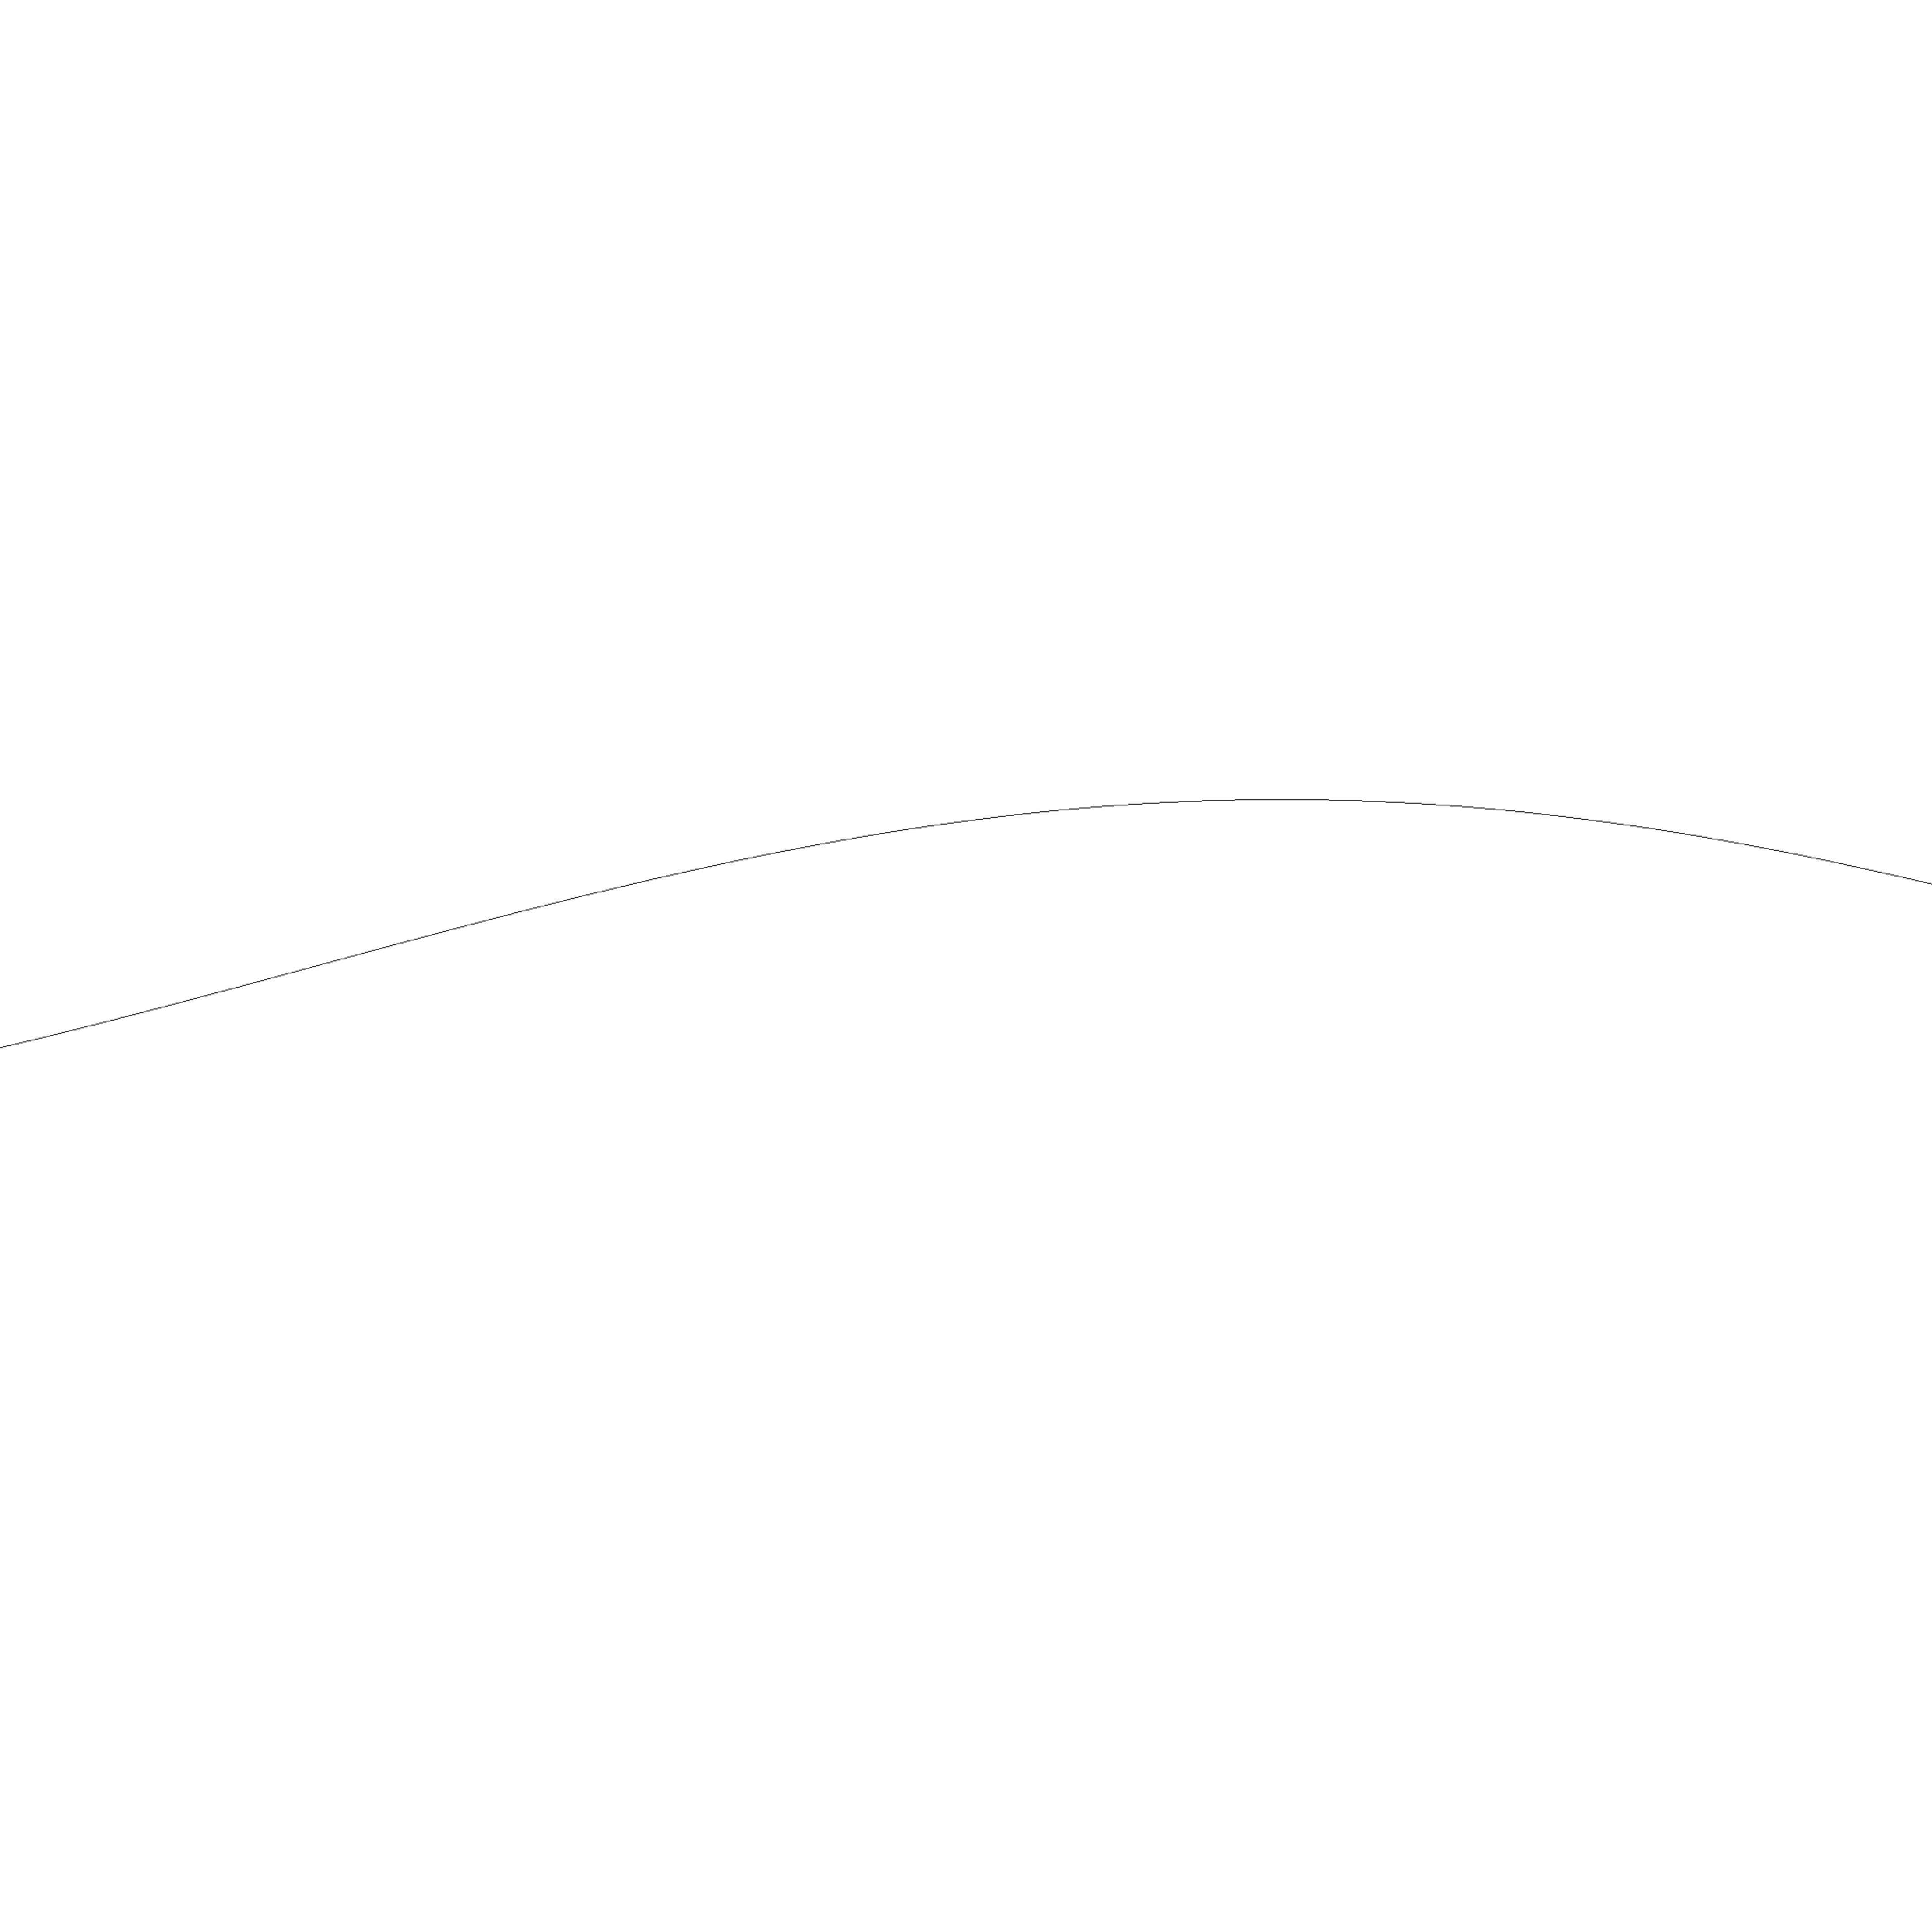
\includegraphics[width=0.88\textwidth]{figs/jet1/vertex.pdf}
	\caption{Second Hough Transform identifies the sinusoid corresponding to the jet vertex.  \label{fig:jet1_vertex}}
	\end{center}
\end{minipage}
\end{figure}

\begin{figure}[!Hhtb]
\begin{minipage}[t]{4.9cm}
\begin{center}
	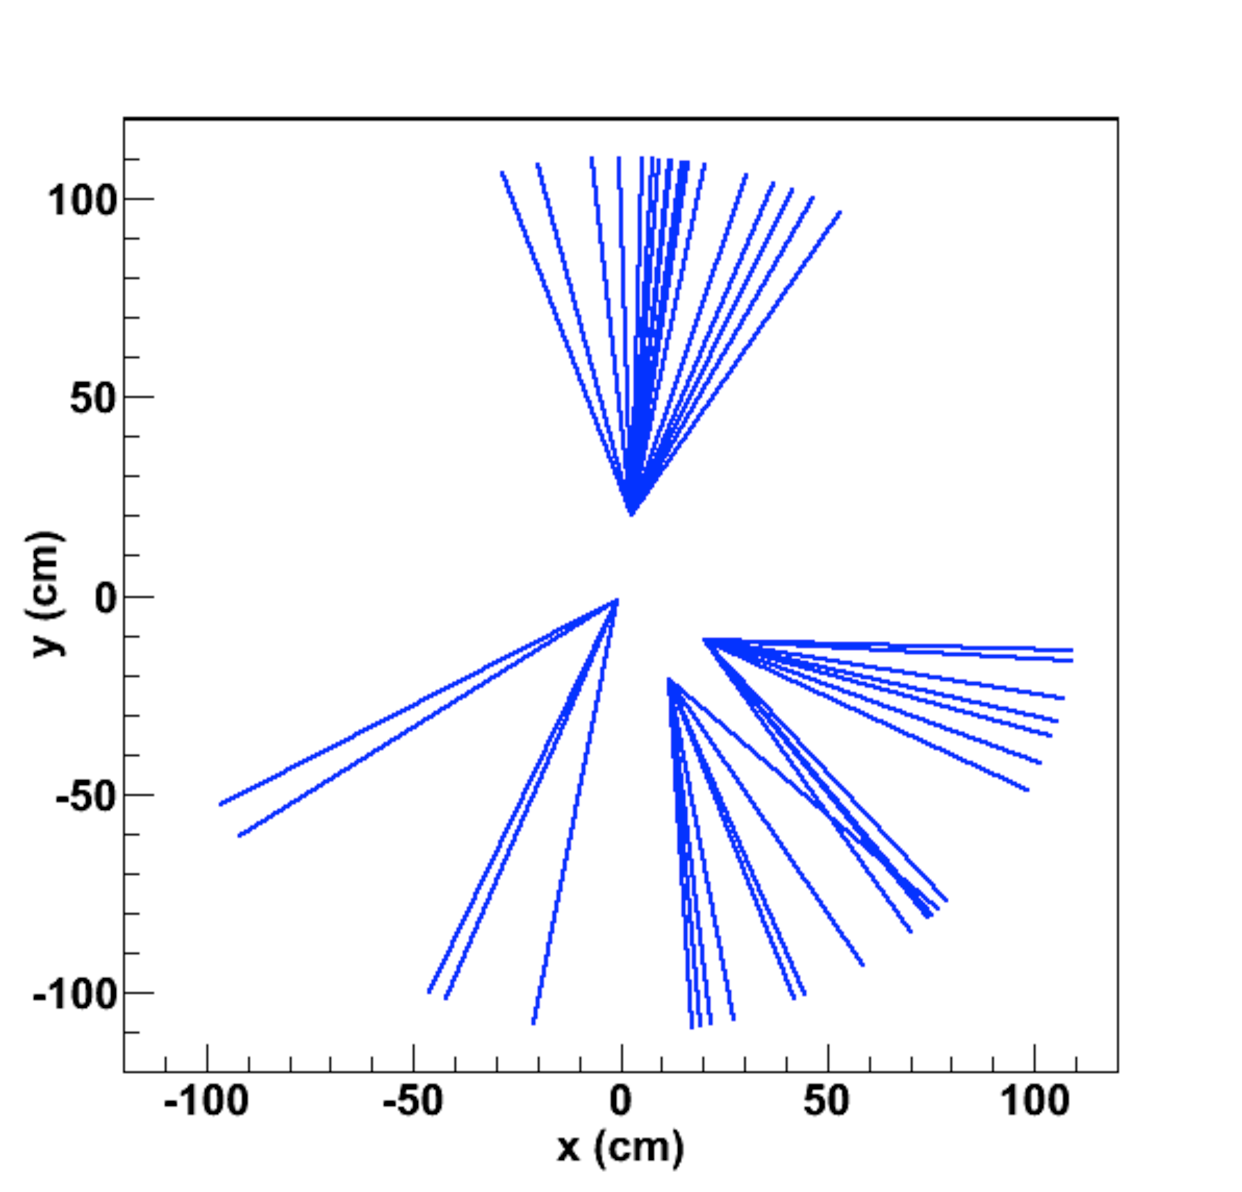
\includegraphics[width=1.\textwidth]{figs/jet2/tracks.pdf}
	\caption{Tracks originating from multiple displaced jets. \label{fig:jet2_tracks}}
	\end{center}
\end{minipage}
\begin{minipage}[t]{4.9cm}
\begin{center}
	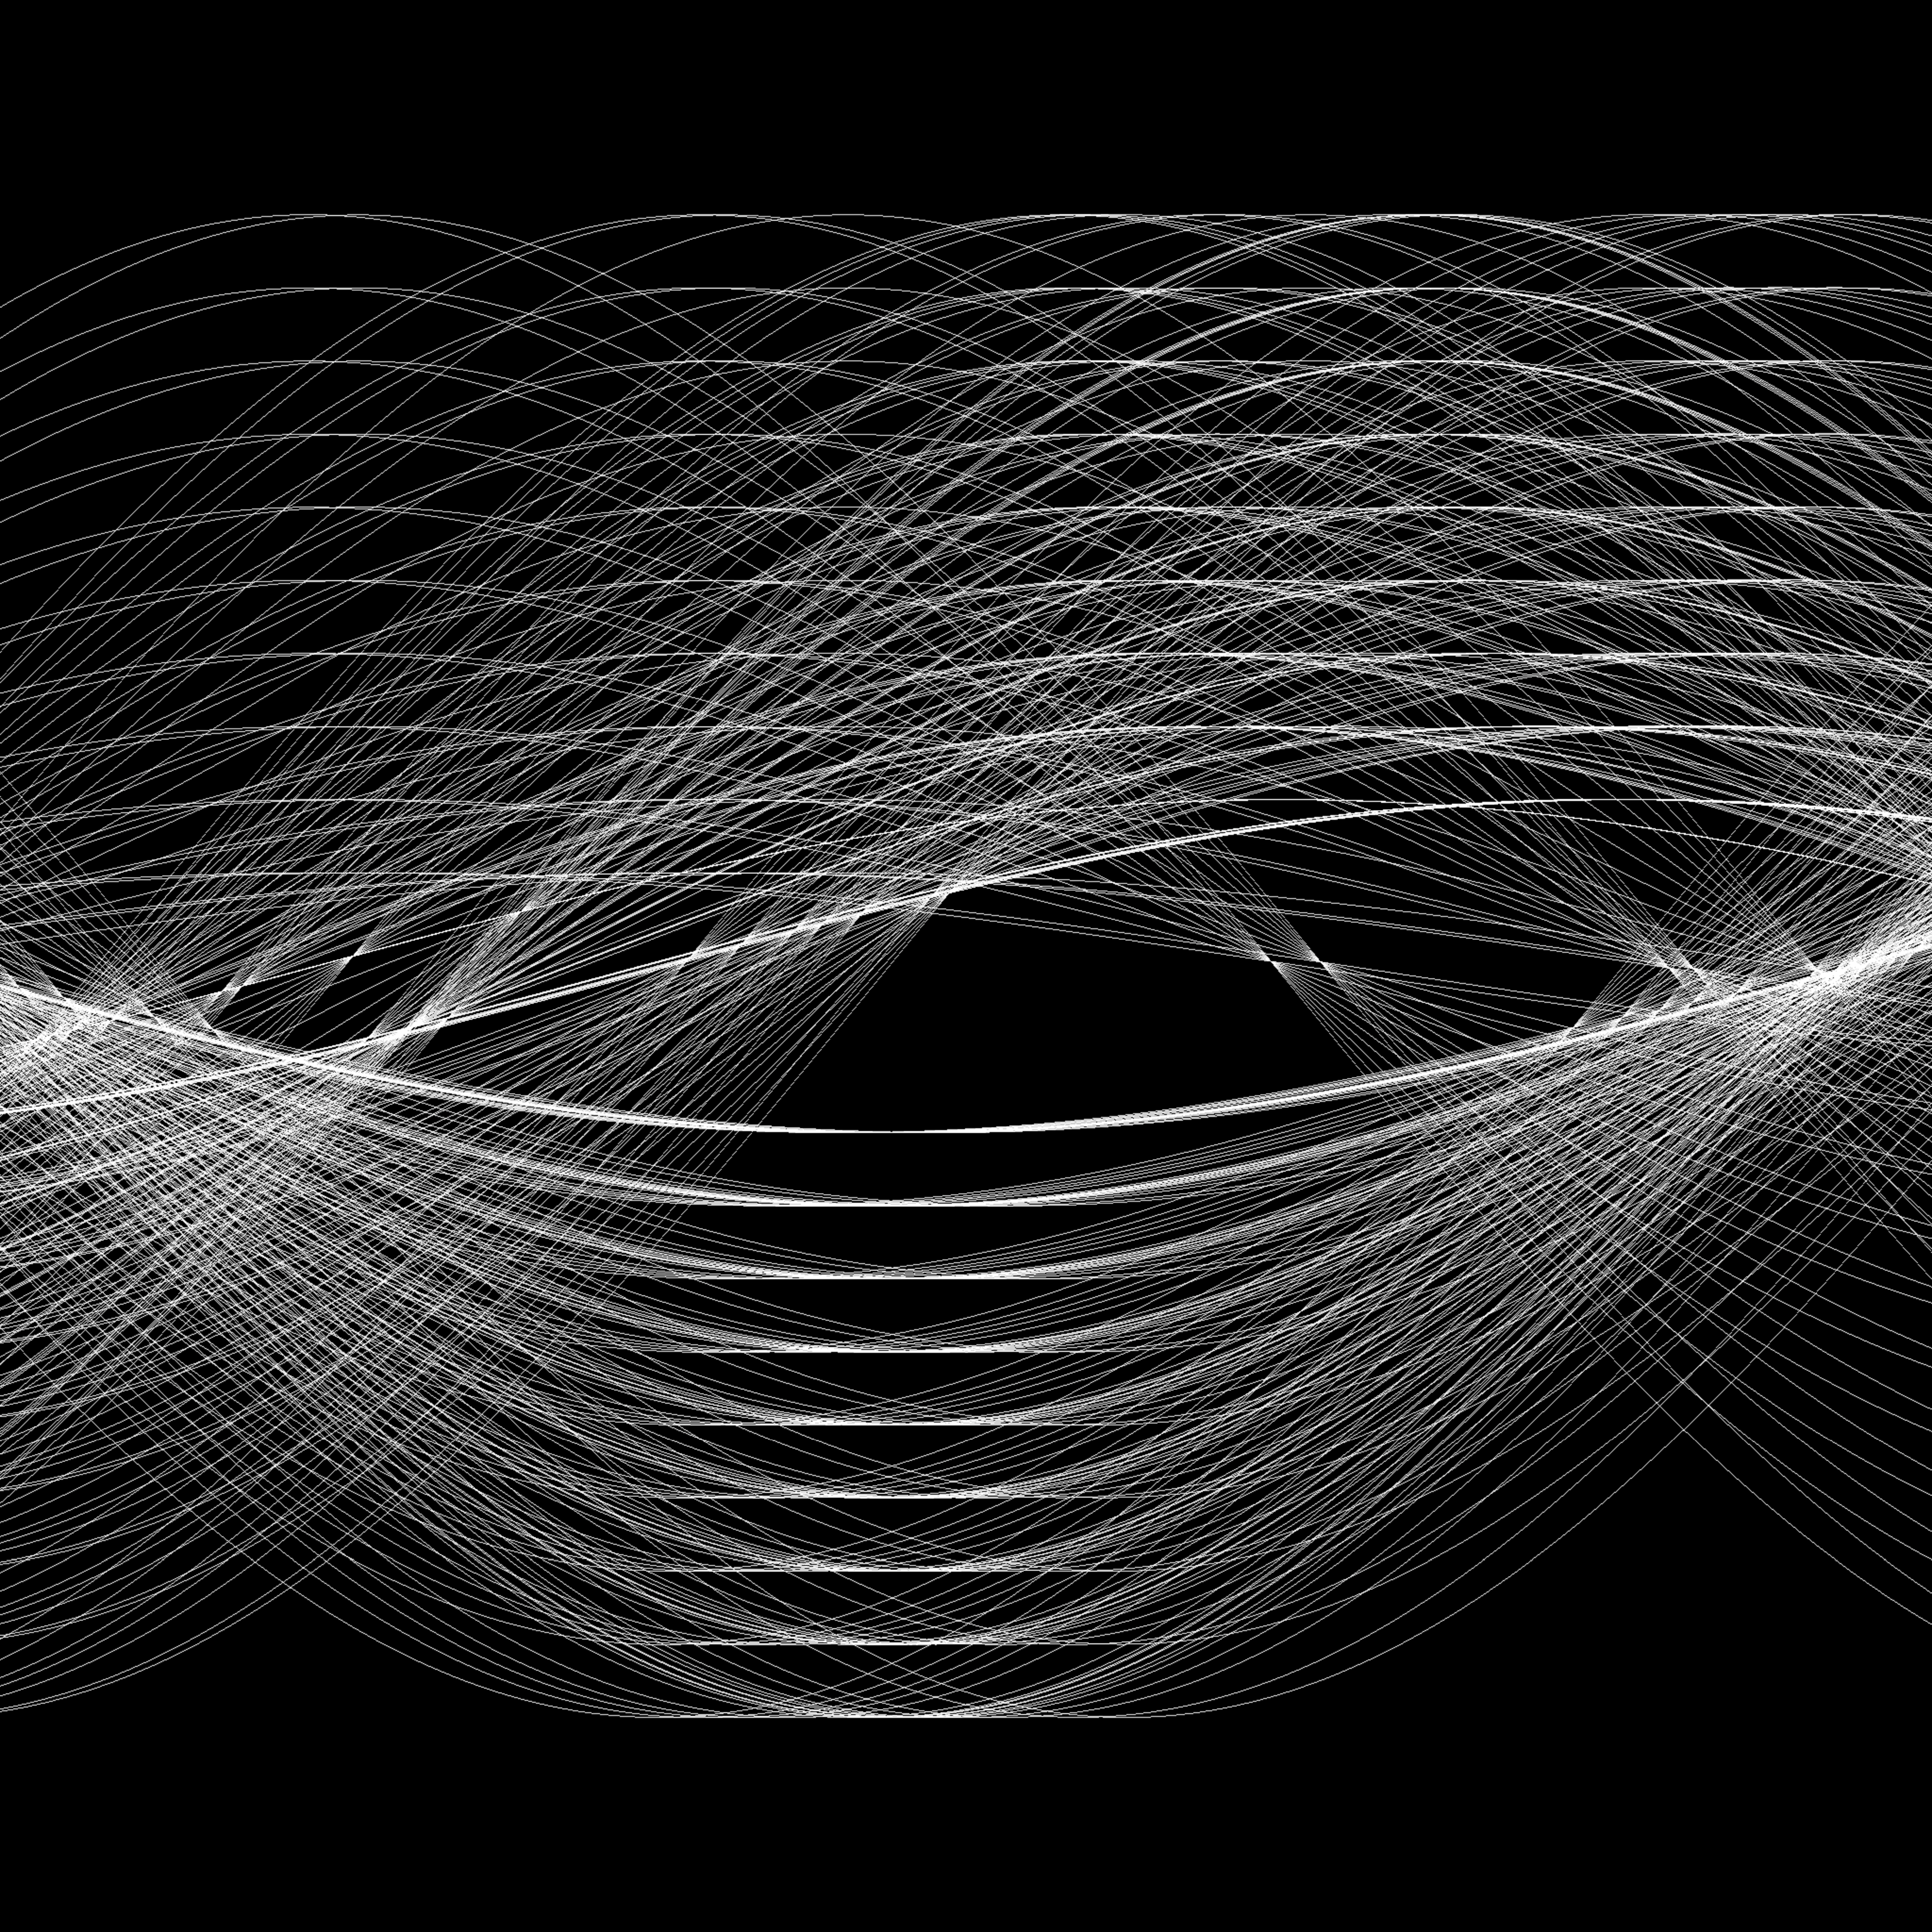
\includegraphics[width=0.88\textwidth]{figs/jet2/accumulator.pdf}
	\caption{Parameter space is difficult to visually interpret.  \label{fig:jet2_accumulator}}
	\end{center}
\end{minipage}
\begin{minipage}[t]{4.9cm}
\begin{center}
	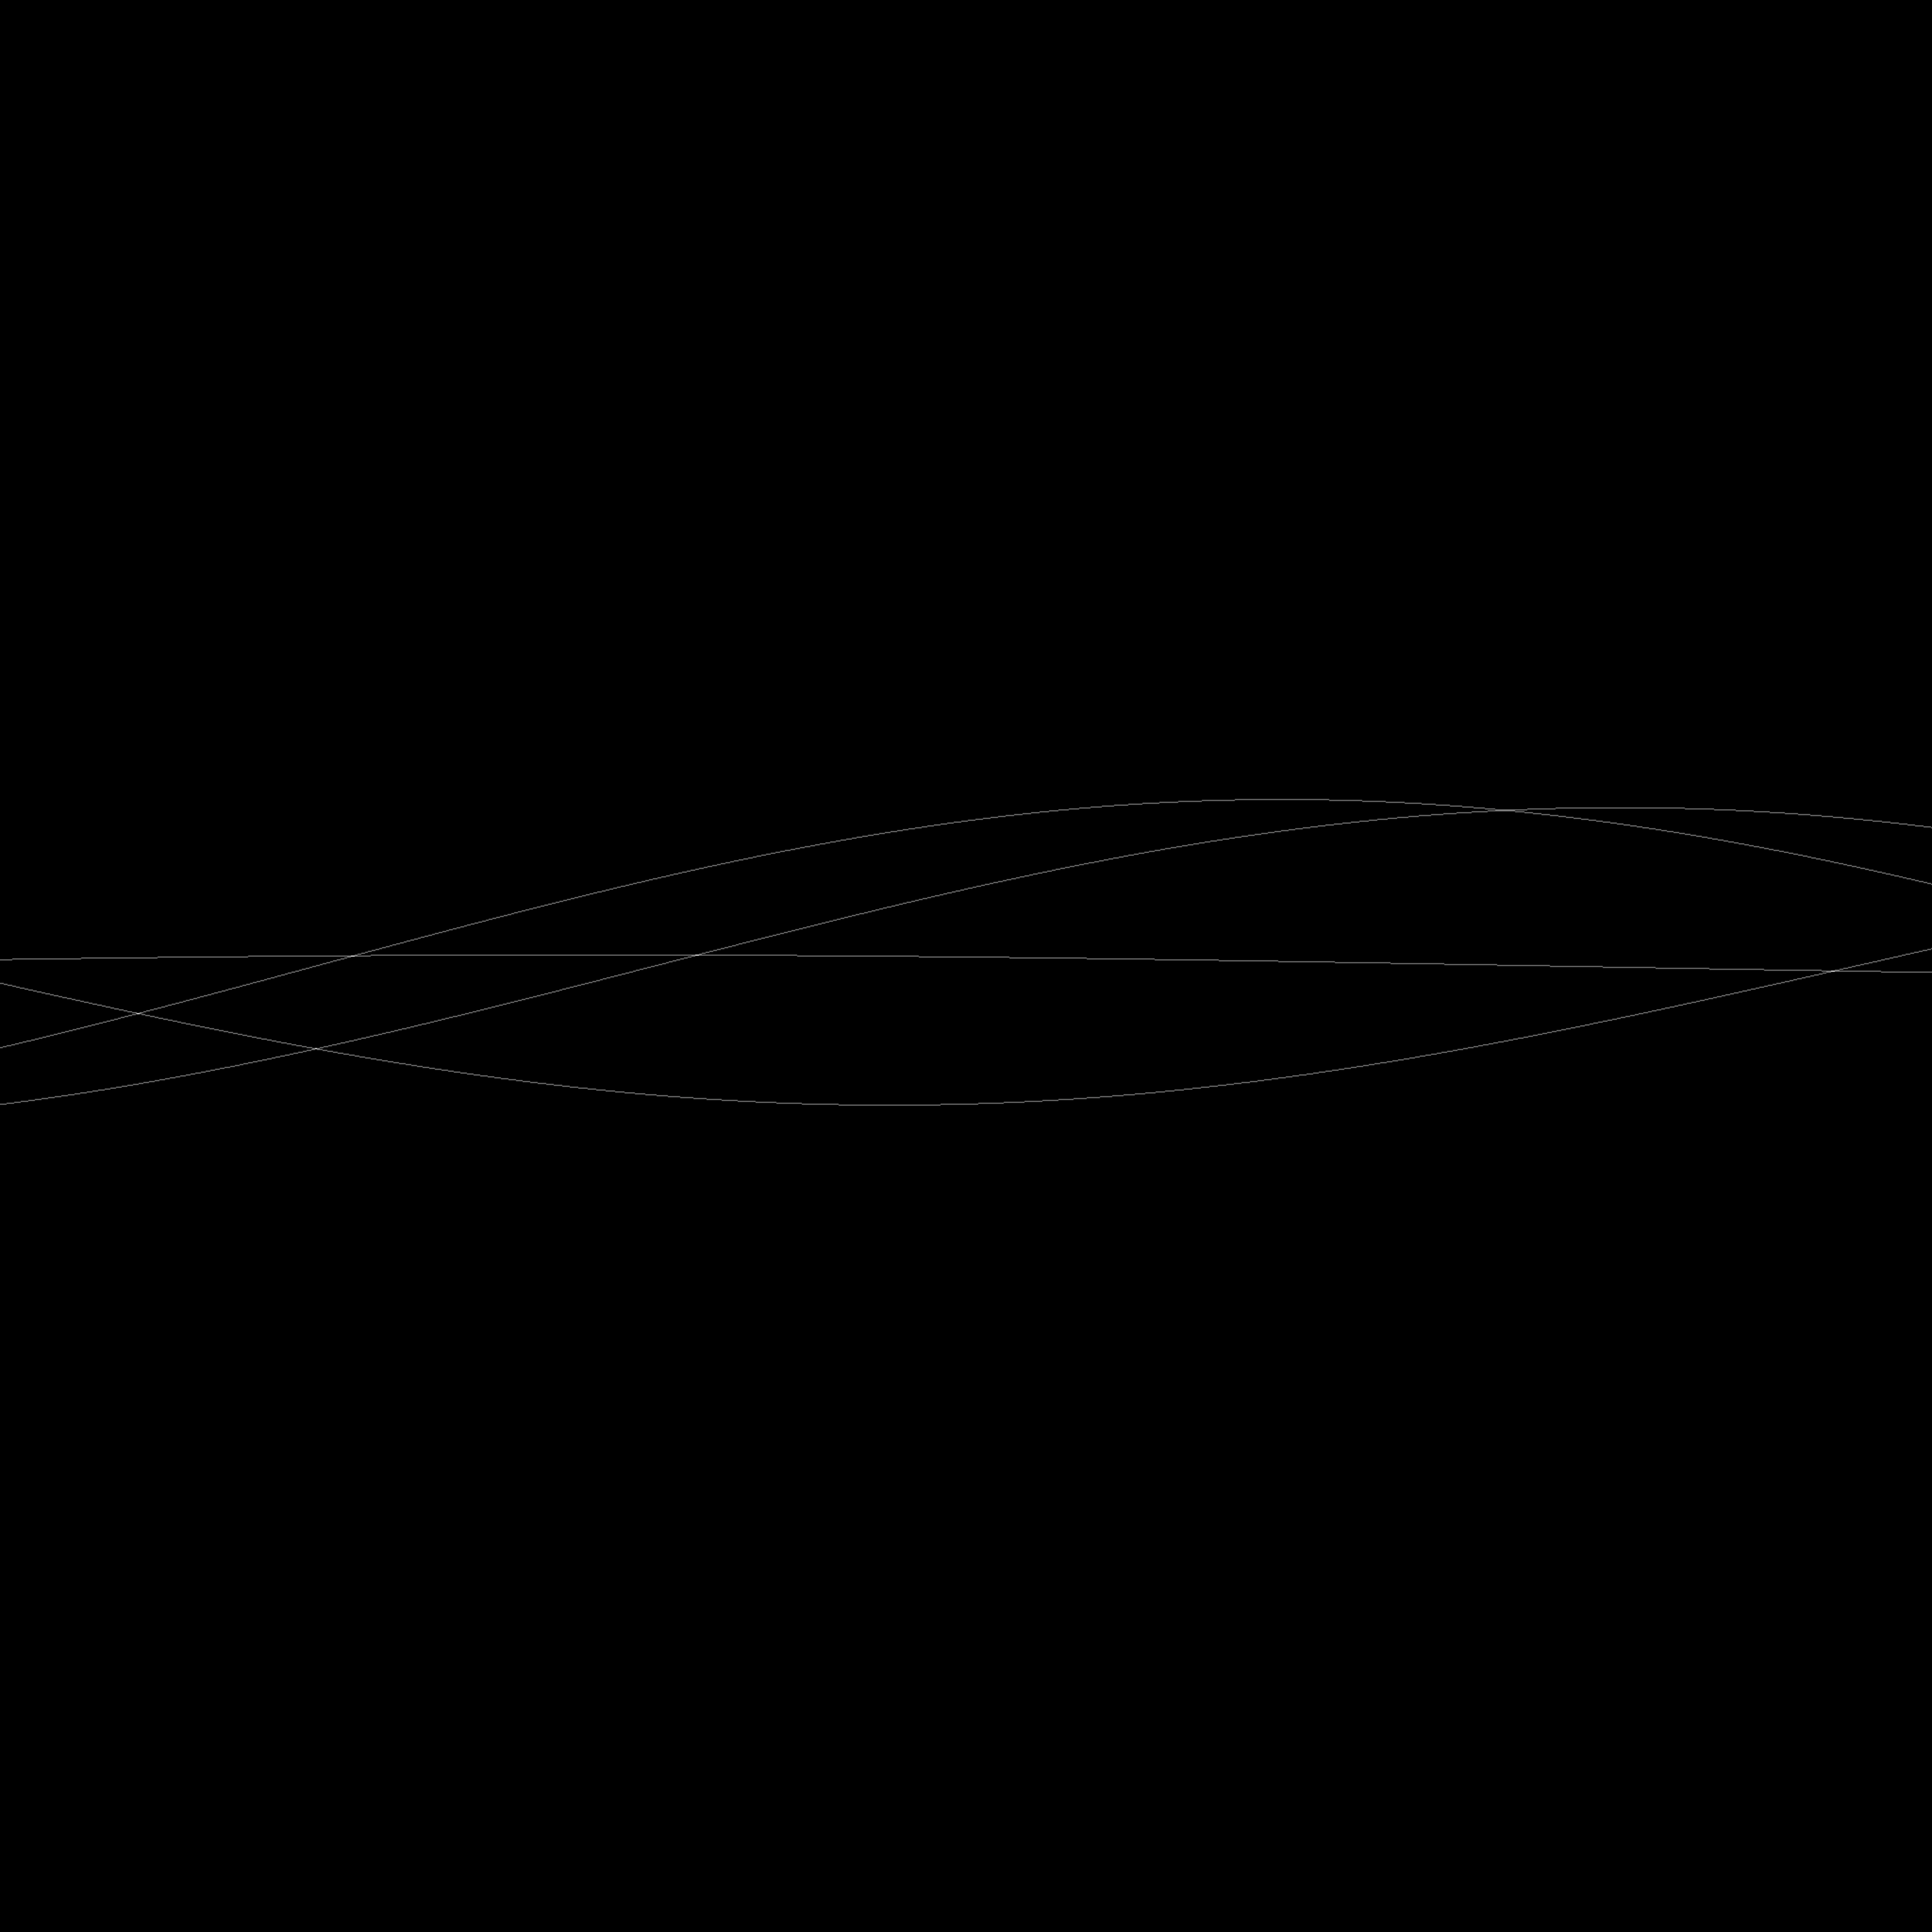
\includegraphics[width=0.88\textwidth]{figs/jet2/vertex.pdf}
	\caption{Second Hough Transform identifies the sinusoids corresponding to the jet vertices.  \label{fig:jet2_vertex}}
	\end{center}
\end{minipage}
\end{figure}

%
\section{Summary}
%

The quest for rare new physics phenomena and the flexibility of the trigger systems of the general purpose detectors at the LHC 
allowed the authors to proposed a GPU enhancement of the trigger systems.  A tracking algoritm based on a machine vision, Hough Transform algorithm provides
a different, complemetary technique  which is a more holistic operating on an entire image as whole. The algorithm not only permits to find simultanouly any
 random orientation of prompt/non prompt tracks but also us to develop new trigger algorithms such as displaced jets or black holes. These new algorithms are smoking guns to 
to new type of topologies  that surley extend the reach of physics at the LHC. This tracking algorithm will not replace the exisiting combinatoric track 
finder but will enhanhance its capabilities on the trigger. The results presented here are our first preliminary results meant to demonstrate the feasibility of the 
algorithm and its potential impact. Even tough it is feasible to complete the testing of the new triggers proposed by the end of the shut down.
Extensive work has to be done to improve tracking efficiency and purity for the general full tracking algorithm. In addition, 
%Possible sentences for future work to better optimize CPU performance:
to better understand the relative performance of CPUs and GPUs we intend to implement vectorization on the CPU to fully utilize the Advanced Vector Extensions (AVX) 
capability present on modern CPUs from Intel and AMD.  Although the GPU might still show a compelling performance advantage for this class of computations, 
the 256 bit AVX capabilities should increase the CPU performance and allow us to better quantify that advantage.


%%%%%%%%%%%%%%%%
% References
%%%%%%%%%%%%%%%%

\begin{thebibliography}{9}

% The citation is wrong pls find the right thing but it is an example
% first is the ATLAS trg tdr
\bibitem{bib:ATLAStrigger_tdr}
ATLAS Collaboration,
\textsl{Technical Design Report for the ATLAS Muon Spectrometer},
CERN/LHCC/97-22, May 1997.

% CMS trg tdr 
\bibitem{bib:CMSTDR2} The CMS Collaboration, 
\emph{CMS, The TriDAS Project, technical design report, Volume 2: Data acquisition and high-level trigger}
CERN LHCC 2002-36, (2002)

% This one is correct 
\bibitem{ATLAS_detector_paper}
The ATLAS collaboration,
\emph{The ATLAS Experiment at the CERN Large Hadron Collider},
JINST {\textbf 3}  S08003 (2008)
%
% this one is wrong put the correct CMS det paper
\bibitem{CMS_detector_paper}
The CMS collaboration,
\emph{The CMS Experiment at the CERN Large Hadron Collider},
JINST {\textbf 3}  S08003 (2008)
%
%correct
\bibitem{bib:CUDA}
J. Sabders, E. Kandrot 
\emph{CUDA by Example},
ISBN 978-0-13-138768-3 Addion-Wesley.

% This one is correct
\bibitem{bib:hiddenvalley} 
M. J. Strassler, K. M. Zurek, 
\emph{Echoes of a hidden valley at hadron colliders},
Phys.Lett.B651:374-379,2007 
%
%fix up the papers below to the right format
\bibitem{bib:HtoLJ} A. Falkowski, J. T. Ruderman, T. Volansky, J. Zupan [arXiv:1002.2952]
%
\bibitem{bib:HMSSM} S. Chang, P. J. Fox, N. Weiner JHEP 0608 (2006) 068
%
\bibitem{bib:HSV}  M. J. Strassler, K. M. Zurek, Phys.Lett.B661:263-267,2008
%
%
\bibitem{bib:TP} The CMS Collaboration, “CMS technical proposal,” CERN LHCC 94-38, 1994.
%
%
\bibitem{bib:TDR1} The CMS Collaboration, “CMS, The TriDAS Project, technical design
report, Volume 1: The trigger systemsm” CERN LHCC 2000-38, 2000.
%
%
\bibitem{bib:TDR2} The CMS Collaboration, “CMS, The TriDAS Project, technical design
report, Volume 2: Data acquisition and high-level trigger,” CERN LHCC 2002-36, 2002.
%
%
\bibitem{bib:HLT} IEEE TRANSACTIONS ON NUCLEAR SCIENCE, VOL. 55, NO. 1, 2008
%
%
\bibitem{bib:HT1}P.V.C. Hough, 
\emph{Machine Analysis of Bubble Chamber Pictures}, 
Proc. Int. Conf. High Energy Accelerators and Instrumentation, 1959
%
%
\bibitem{bib:HT2} Gonzalez, R.C. and Woods, R.E., 
\emph{Digital Image Processing},
Prentice Hall, 1993.

\end{thebibliography}

\end{document}
